%%%%%%%%%%%%%%%%%%%%%%%%%%%%%%%%%%%%%%%%%%%%%%%%%
%%%%       Juniormar Organista 	     	%%%%
%%%%%%%%%%%%%%%%%%%%%%%%%%%%%%%%%%%%%%%%%%%%%%%%%
\documentclass[10pt, aspectratio=169]{beamer}
\usetheme[
%%% options passed to the outer theme
%    progressstyle=fixedCircCnt,   %either fixedCircCnt, movCircCnt, or corner
%    rotationcw,          % change the rotation direction from counter-clockwise to clockwise
%    shownavsym          % show the navigation symbols
]{AAUsimple}

\usepackage[utf8]{inputenc}
\usepackage[portuguese]{babel}
\usefonttheme{serif}
\usepackage{pgfgantt}
\usepackage{amsthm,amsmath,amssymb,amsfonts,latexsym,cancel}
\usepackage{mathptmx}
\usepackage{eulervm}
\usepackage{helvet}
%\usepackage{lmodern}
\usepackage{tikz}
\usepackage{multimedia}
%\usepackage{movie15}
\usepackage{ragged2e}
\usepackage{units}
%\usepackage[skins,theorems]{tcolorbox}
\usepackage{stmaryrd}
\usepackage{fancybox}
% \usepackage[backend=bibtex,style=authoryear]{biblatex}

\usepackage{natbib}
% \usepackage{biblatex}

\usepackage{hyperref}
\usepackage{textpos}
%\usepackage{wrapfig}
\usepackage[most]{tcolorbox}
\usepackage{empheq}
% \usepackage{subcaption}
\usepackage{comment}
\usepackage{subfigure}
\usepackage{rotating}
\usepackage{xcolor}
\usepackage{transparent}
\usepackage{verbatim}
\usepackage{color}
\usepackage{multicol,caption}
\usepackage[all,knot,arc,import,poly]{xy}
\usepackage{colortbl}
\usepackage{slashbox}
\usepackage{multirow}
\usepackage{mathtools}
\usepackage[all]{xy}
\usepackage{color}
\usepackage[T1]{fontenc}
\usepackage{booktabs}

\graphicspath{{images/}}
\DeclareMathOperator{\trace}{tr}
\renewcommand{\vec}[1]{\mathbf{#1}}
\newcommand{\tab}[1]{\hspace{.1\textwidth}\rlap{#1}}
\newcommand{\norm}[1]{\left\lVert#1\right\rVert}
\newcommand*{\defeq}{\mathrel{\vcenter{\baselineskip0.5ex \lineskiplimit0pt
                     \hbox{\scriptsize.}\hbox{\scriptsize.}}}%
                     =}

\newcommand{\Bl}{\textcolor{red}{\rule{5ex}{1ex}}}
\newcommand{\Gr}{\textcolor{black}{\rule{5ex}{1ex}}}
\newcommand{\surgr}{\nabla_{\scriptscriptstyle{\Gamma}}}
\newcommand{\surlp}{\Delta_{\scriptscriptstyle{\Gamma}}}
\newcommand{\Gam}{\scriptscriptstyle{\Gamma}}
\newcommand*{\Scale}[2][4]{\scalebox{#1}{$#2$}}%

\theoremstyle{remark}
\newtheorem{obgeral}{Objetivo geral}
\newtheorem{obesp}{Objetivos específicos}
\newtheorem{Just}{Justificativas}
\newtheorem{prop}{Proposition}
\newtheorem{teo}{Theorem}
\newtheorem{lema}{Lema}
\newtheorem{defi1}{Definição 1.}
\newtheorem{defi2}{Definição 2.}
\definecolor{blue}{rgb}{0,0,255}

\newcounter{saveenumi}
\newcommand{\seti}{\setcounter{saveenumi}{\value{enumi}}}
\newcommand{\conti}{\setcounter{enumi}{\value{saveenumi}}}

% Definição dos estilos dos nós
\tikzstyle{caixa} = [rectangle, rounded corners, minimum width=3cm, minimum height=1cm, text centered, draw=black, fill=blue!20]
\tikzstyle{processo} = [rectangle, minimum width=3cm, minimum height=1cm, text centered, draw=black, fill=gray!20]
\tikzstyle{seta} = [thick,->,>=stealth]

% colored hyperlinks
\newcommand{\chref}[2]{%
  \href{#1}{{\usebeamercolor[bg]{AAUsimple}#2}}%
}
%\usetikzlibrary{arrows}
\title[Métodos das Soluções Manufaturadas para Fluidos Viscoelásticos]{Verificação de Código de Simulação Numérica de Escoamentos de Fluidos Viscoelásticos Através do Método de Soluções Manufaturadas}
%\subtitle{v.\ 1.2.1}  % could also be a conference name
%\date{18 de Novembro de 2014}

\author[Organista, J.]{
  Juniormar Organista
}

% - Give the names in the same order as they appear in the paper.
% - Use the \inst{?} command only if the authors have different
%   affiliation. See the beamer manual for an example

\institute[ICMC]{
    \textbf{Orientador:} Prof. Dr. Leandro Franco de Souza\\
    \vspace{0.1cm}
    Instituto de Ciências Matemáticas e de Computação\\
    Universidade de São Paulo
}
\date{27 de fevereiro de 2025}
%\date{\today}
% specify a logo on the titlepage (you can specify additional logos an include them in 
% institute command below
\pgfdeclareimage[height=0.8cm]{titlepagelogo}{AAUgraphics/logohorizontal} % placed on the title page
%\pgfdeclareimage[height=1.5cm]{titlepagelogo2}{AAUgraphics/streamslines} % placed on the title page
\titlegraphic{% is placed on the bottom of the title page
  \pgfuseimage{titlepagelogo}
%  \hspace{1cm}\pgfuseimage{titlepagelogo2}
}

% Definir a imagem de fundo para todos os slides, exceto o primeiro
\AtBeginSection[]{
	\usebackgroundtemplate{
		\begin{tikzpicture}
			\useasboundingbox (0,0) rectangle (\paperwidth,\paperheight);
			% Define a imagem de fundo com opacidade ajustada
			\node[opacity=0.1] at (current page.center) {
				\includegraphics[width=\paperwidth,height=\paperheight]{AAUgraphics/streamslines}
			};
		\end{tikzpicture}
	}
}

%%%%%%%%%%%%%---------------%%%%%%%%%%%%%%%%%%%%%%%%%%%%%%%%%%
%%%%%%%%%%%%%---------------%%%%%%%%%%%%%%%%%%%%%%%%%%%%%%%%%%
\begin{document}
% the titlepage

{\aauwavesbg%
\begin{frame}[plain,noframenumbering] % the plain option removes the header from the title page
  \titlepage
\end{frame}
}

%%%%%%%%%%%%%%%%%%%%%%%%%%%%%%%%%%%%%%%%%%%%%%%%%%%%%%%%%%%%%%
\begin{frame}{Organização da apresentação}{}
\tableofcontents
\end{frame}

%%%%%%%%%%%%%%%%%%%%%%%%%%%%%%%%%%%%%%%%%%%%%%%%%%%%%%%%%%%%%%
%%% Motivação
%%%%%%%%%%%%%%%%%%%%%%%%%%%%%%%%%%%%%%%%%%%%%%%%%%%%%%%%%%%%%%
%%%%%%%%%%%%%%%%%%%%%%%%%%%%%%%%%%%%%%%%%%%%%%%%%%%%%%%%%%%%%%
\section{Motivação}
%%%%%%%%%%%%%%%%%%%%%%%%%%%%%%%%%%%%%%%%%%%%%%%%%%%%%%%%%%%%%%

%%%%%%%%%%%%%%%%%%%%%%%%%%%%%%%%%%%%%%%%%%%%%%%%%%%%%%%%%%%%%%
\begin{frame}{Aplicações Industriais dos Fluidos Viscoelásticos}
\begin{itemize}
    \item CFD ferramenta essencial para simulações confiáveis;
    \item Fluidos viscoelásticos desempenham papel crucial em processos industriais;
    \item Aplicações incluem processamento de polímeros, injeção de plásticos e extração de petróleo;
    \item Desafios na modelagem devido à resposta não linear ao estresse e deformação;
    \item Métodos numéricos avançados garantem previsões precisas do comportamento dos fluidos;
    \item Permite análises detalhadas em vista da experimentação física;
    \item Necessidade de Verificação e Validação rigorosas;
\end{itemize}
\end{frame}

%%%%%%%%%%%%%%%%%%%%%%%%%%%%%%%%%%%%%%%%%%%%%%%%%%%%%%%%%%%%%%
\begin{frame}{Motivação}
\begin{center}
    \begin{tikzpicture}[node distance=2cm]
        % Nó principal
        \node (fluido) [caixa] {Fluidos};
        % Divisão: Newtonianos e Não Newtonianos
        \node (newtoniano) [processo, below left=1cm and 1cm of fluido] {Newtonianos};
        \node (naonewtoniano) [processo, below right=1cm and 1cm of fluido] {Não Newtonianos};
        % Conexões principais
        \draw [seta] (fluido.south) -- ++(-1,-0.5) -| (newtoniano.north);
        \draw [seta] (fluido.south) -- ++(1,-0.5) -| (naonewtoniano.north);
        % Subdivisões dos fluidos não newtonianos
        \node (pseudoplasticos) [processo, below left=1cm and 0.5cm of naonewtoniano] {Pseudoplásticos};
        \node (dilatantes) [processo, below right=1cm and 0.5cm of naonewtoniano] {Dilatantes};
        \node (viscoelasticos) [processo, below=2.5cm of naonewtoniano] {\textcolor{red}{Viscoelásticos}};
        % Conexões das subclasses
        \draw [seta] (naonewtoniano.south) -- ++(-0.5,-0.5) -| (pseudoplasticos.north);
        \draw [seta] (naonewtoniano.south) -- ++(0.5,-0.5) -| (dilatantes.north);
        \draw [seta] (naonewtoniano.south) -- (viscoelasticos.north);
    \end{tikzpicture}
\end{center}
\end{frame}

%%%%%%%%%%%%%%%%%%%%%%%%%%%%%%%%%%%%%%%%%%%%%%%%%%%%%%%%%%%%%%
\begin{frame}{Modelos Reológicos para Fluidos Viscoelásticos}
\begin{itemize}
    \item \textbf{UCM (Upper Convected Maxwell)}: \cite{beris1987spectral}
    \begin{itemize}
        \item Modelo mais simples para fluidos viscoelásticos;
        \item Útil para escoamentos com baixa taxa de cisalhamento;
    \end{itemize}
    \item \textbf{Oldroyd-B}: \cite{brasseur1998time}
    \begin{itemize}
        \item Generalização do modelo UCM;
        \item Aplicável a soluções poliméricas diluídas;
    \end{itemize}
    \item \textbf{Giesekus}: \cite{giesekus1962}
    \begin{itemize}
        \item Baseado em sistemas de esferas e molas;
        \item Considera efeito de anisotropia na força de arrasto;
        \item Adiciona termos não lineares ao tensor de tensões;
    \end{itemize}
    \item \textbf{LPTT (Linear Phan-Thien-Tanner)}: \cite{phan-thien77}
    \begin{itemize}
        \item Baseado na teoria de redes de polímeros fundidos;
        \item Aplica-se a materiais com altas taxas de cisalhamento;
    \end{itemize}
    \item \textbf{Maxwell}: \cite{Kaye62}
    \begin{itemize}
        \item Modelo integral clássico para a descrição de fluidez em materiais viscoelásticos;
    \end{itemize}
    \item \textbf{K-BKZ (Kaye-Bernstein-Kearsley-Zapas)}: \cite{luo88}
    \begin{itemize}
        \item Modelo integral que estende a formulação de Maxwell para materiais com efeitos não lineares;
        \item Aplicável a simulações avançadas de fluxo de polímeros.
    \end{itemize}
\end{itemize}
\end{frame}

%%%%%%%%%%%%%%%%%%%%%%%%%%%%%%%%%%%%%%%%%%%%%%%%%%%%%%%%%%%%%%
\begin{frame}{Desafios na Simulação de Fluidos Viscoelásticos}
\begin{itemize}
    \item Equações constitutivas complexas dificultam a modelagem;
    \item Métodos numéricos permitem redução de custos e maior precisão;
    \item Principais desafios computacionais:
    \begin{itemize}
        \item Implementação de equações não lineares;
        \item Convergência e estabilidade numérica;
        \item Tratamento adequado de condições de contorno;
    \end{itemize}
\end{itemize}
\end{frame}

%%%%%%%%%%%%%%%%%%%%%%%%%%%%%%%%%%%%%%%%%%%%%%%%%%%%%%%%%%%%%%
\begin{frame}{Motivação}
\begin{itemize}
    \item Confiabilidade e precisão são essenciais na modelagem computacional;
    \item Importância da Verificação e Validação (VV) na simulação numérica;
    \item Diferentes perspectivas sobre VV: \cite{oberkampftech} e \cite{Roache2002};
    \item Métodos de Verificação de Código, incluindo o Método das Soluções Manufaturadas (MMS);
    \item Aplicação da MMS em trabalhos como \cite{shih1989effects} e \cite{oberkampftech};
\end{itemize}
\end{frame}

%%%%%%%%%%%%%%%%%%%%%%%%%%%%%%%%%%%%%%%%%%%%%%%%%%%%%%%%%%%%%%
\begin{frame}{Verificação x Validação}
\begin{itemize}
    \item \textbf{Verificação}: Avalia se o código computacional está correto
    \begin{itemize}
        \item Testes com soluções analíticas e casos de referência;
        \item Identificação de erros e inconsistências numéricas;
    \end{itemize}
    \item \textbf{Validação}: Compara resultados numéricos com dados experimentais
    \begin{itemize}
        \item Mede a precisão da simulação em relação ao mundo real;
    \end{itemize}
    \item Técnica essencial para Verificação e Validação de códigos numéricos;
    \item Simulações de fluidos viscoelásticos exigem abordagens robustas;
\end{itemize}
\end{frame}

%%%%%%%%%%%%%%%%%%%%%%%%%%%%%%%%%%%%%%%%%%%%%%%%%%%%%%%%%%%%%%
\begin{frame}{Objetivo do Trabalho}
\begin{itemize}
    \item Desenvolver uma \textbf{Solução Manufaturada} para verificação de código numérico para escoamentos viscoelásticos.
    \item Foco nos modelos constitutivos:
    \begin{itemize}
        \item UCM (Upper Convected Maxwell);
        \item Oldroyd-B;
        \item Giesekus;
        \item LPTT (Linear Phan-Thien-Tanner);
    \end{itemize}
    \item Avaliação da precisão do código e correção de possíveis inconsistências.
    \item Contribuição para a confiabilidade e robustez de códigos aplicados a fluidos viscoelásticos.
\end{itemize}
\end{frame}

%%%%%%%%%%%%%%%%%%%%%%%%%%%%%%%%%%%%%%%%%%%%%%%%%%%%%%%%%%%%%%
%%% Formulação
%%%%%%%%%%%%%%%%%%%%%%%%%%%%%%%%%%%%%%%%%%%%%%%%%%%%%%%%%%%%%%
%%%%%%%%%%%%%%%%%%%%%%%%%%%%%%%%%%%%%%%%%%%%%%%%%%%%%%%%%%%%%%
\section{Formulação Matemática}
%%%%%%%%%%%%%%%%%%%%%%%%%%%%%%%%%%%%%%%%%%%%%%%%%%%%%%%%%%%%%%

%%%%%%%%%%%%%%%%%%%%%%%%%%%%%%%%%%%%%%%%%%%%%%%%%%%%%%%%%%%%%%
\subsection{Equações Governantes}
%%%%%%%%%%%%%%%%%%%%%%%%%%%%%%%%%%%%%%%%%%%%%%%%%%%%%%%%%%%%%%

%%%%%%%%%%%%%%%%%%%%%%%%%%%%%%%%%%%%%%%%%%%%%%%%%%%%%%%%%%%%%%
\begin{frame}{Equações Governantes}
Escoamentos incompressíveis e isotérmicos são governados pela equação de continuidade, que assegura a conservação da massa:
\begin{equation}\label{eq_conservacao_massa}
    \nabla \cdot \mathbf{u} = 0,
\end{equation}
e pela equação de quantidade de movimento, que representa a conservação de momentum:
\begin{equation}\label{eq_conservacao_momentum}
    \rho \left( \frac{\partial \mathbf{u}}{\partial t} + \nabla \cdot (\mathbf{u} \mathbf{u}) \right) = \nabla \cdot \sigma,
\end{equation}
onde $\rho$ é a massa específica do fluido (densidade), $\mathbf{u}$ é o vetor de velocidade e $t$ é o tempo. A variável $\sigma$ é o tensor de tensões totais, definido por:
\begin{equation}\label{eq_tensoes_totais}
    \sigma = \tau - p \mathbf{I},
\end{equation}
onde $p$ é a pressão, $\mathbf{I}$ é o tensor identidade, e $\tau$ é o tensor de tensões extra-simétrico
\end{frame}

%%%%%%%%%%%%%%%%%%%%%%%%%%%%%%%%%%%%%%%%%%%%%%%%%%%%%%%%%%%%%%
\begin{frame}{Equações Governantes}
Para fluidos newtonianos, o tensor de tensões $\tau$ é proporcional ao tensor taxa de deformação $\mathbf{D}$, conforme a relação linear:
\begin{equation}\label{eq_tensoes_totais_newtoniano}
    \tau = 2 \mu_s \mathbf{D},
\end{equation}
onde $\mu_s$ é a viscosidade dinâmica do fluido e $\mathbf{D}$ é o tensor taxa de deformação, dado por:
\begin{equation}\label{eq_taxa_deformacao_newtoniano}
    \mathbf{D} = \frac{1}{2}(\nabla \mathbf{u} + \nabla\mathbf{u}^{T} ).
\end{equation}
Para fluidos não newtonianos, o tensor extra-tensões simétrico é definido como a soma da contribuição newtoniana (viscosa) e da contribuição não newtoniana (elástica) \cite{RAJAGOPALAN1990}, que é dado por:
\begin{equation}\label{eq_tensoes_totais_nao_newtoniano}
    \tau=2 \mu_s D+T,
\end{equation}
onde $\mu_s$ é a viscosidade do solvente newtoniano, $D$ é o tensor taxa de deformação definido pela Equação \eqref{eq_taxa_deformacao_newtoniano} e $T$ é o tensor extra-tensão (simétrico) que representa a contribuição não newtoniana do fluido.
\end{frame}

%%%%%%%%%%%%%%%%%%%%%%%%%%%%%%%%%%%%%%%%%%%%%%%%%%%%%%%%%%%%%%
\begin{frame}{Equações Governantes}
O sistema de equações equação de quantidade de movimento para um fluido viscoelástico e a equação constitutiva $LPOG$ adotada para a modelagem do comportamento de fluidos viscoelásticos, apresentada por \cite{furlan2022linear}, é dada por

\begin{equation}\label{eq_conservacao_massa_sistema}
    \nabla \cdot \mathbf{u} = 0,
\end{equation}
\begin{equation}
    \begin{split}
        \rho \left( \frac{\partial \mathbf{u}}{\partial t} + \nabla \cdot (\mathbf{uu}) \right) = -\nabla p + \mu_s \nabla^2 \mathbf{u} + \nabla \cdot \mathbf{T}.
    \end{split}\label{eq_conservacao_momentum_nao_newtoniano_sistema}
\end{equation}
\begin{equation}
    \begin{split}
        f(\mathbf{T})\mathbf{T} + \lambda \left(\frac{\partial \mathbf{T}}{\partial t} + \mathbf{u} \cdot \nabla \mathbf{T} - \mathbf{T} \cdot\nabla \mathbf{u} - \nabla \mathbf{u}^T \cdot \mathbf{T} \right) + \xi\lambda (\mathbf{D} \cdot \mathbf{T} + \mathbf{T} \cdot \mathbf{D}) + \frac{\alpha_G \lambda}{\mu_p} (\mathbf{T} \cdot \mathbf{T}) = 2 \mu_p \mathbf{D},
    \end{split}\label{eq_tensores_lpog_sistema}
\end{equation}
onde $\mu_p$ é o coeficiente de viscosidade polimérica, $\lambda$ representa o tempo de relaxação do fluido, e $\alpha_G$ é o parâmetro de mobilidade que regula o comportamento de afinamento por cisalhamento do fluido e
\begin{equation*}
    f(\mathbf{T}) = 1 + \frac{\epsilon \lambda}{\mu_p} \textbf{tr}(\mathbf{T})
\end{equation*}
\end{frame}

%%%%%%%%%%%%%%%%%%%%%%%%%%%%%%%%%%%%%%%%%%%%%%%%%%%%%%%%%%%%%%
\begin{frame}{Equações Governantes}
Assim na equação constitutiva denominada LPOG, equação \eqref{eq_tensores_lpog_sistema}, é possível derivar quatro modelos viscoelásticos distintos. Para cada modelo, basta realizar as seguintes substituições:
\begin{itemize}
    \item Modelo UCM: $\alpha_G = \xi = \epsilon = 0$ ($\mu_s = 0$); 
    \item Modelo Oldroyd-B: $\alpha_G = \xi = \epsilon = 0$;
    \item Modelo de Giesekus: $\xi = \epsilon = 0$;
    \item Modelo LPTT: $\alpha_G = 0$.
\end{itemize}
\end{frame}

%%%%%%%%%%%%%%%%%%%%%%%%%%%%%%%%%%%%%%%%%%%%%%%%%%%%%%%%%%%%%%
\subsection{Adimensionalização}
%%%%%%%%%%%%%%%%%%%%%%%%%%%%%%%%%%%%%%%%%%%%%%%%%%%%%%%%%%%%%%

%%%%%%%%%%%%%%%%%%%%%%%%%%%%%%%%%%%%%%%%%%%%%%%%%%%%%%%%%%%%%%
\begin{frame}{Adimensionalização}
Considere as seguintes mudanças de variáveis:
\begin{align*}
    \mathbf{x}^*=\frac{\mathbf{x}}{L},\quad \mathbf{u}^*=\frac{\mathbf{u}}{U},\quad \mathbf{t}^*=\frac{t U}{L},\quad \rho^*=\frac{\rho}{p U^2},\quad \tau^*=\frac{\tau}{\rho U^2},\quad \mathbf{T}^*=\frac{\mathbf{T}}{\rho U^2},
\end{align*}
onde $L$ representa a metade da largura do canal e $U$ a escala de velocidade. Após essas substituições nas equações \eqref{eq_conservacao_massa_sistema}, \eqref{eq_conservacao_momentum_nao_newtoniano_sistema} e \eqref{eq_tensores_lpog_sistema}, obtêm-se as equações governantes na forma adimensional:
\end{frame}

%%%%%%%%%%%%%%%%%%%%%%%%%%%%%%%%%%%%%%%%%%%%%%%%%%%%%%%%%%%%%%
\begin{frame}{Adimensionalização}
\begin{equation}
    \begin{split}
        \nabla \cdot \mathbf{u} = 0,
    \end{split}\label{eq_conservacao_massa_admensional}
\end{equation}
\begin{equation}
    \begin{split}
        \frac{\partial \mathbf{u}}{\partial t} + \nabla \cdot (\mathbf{uu}) = -\nabla p + \frac{\beta_{nn}}{Re} \nabla^2 \mathbf{u} + \nabla \cdot \mathbf{T},
\end{split}\label{eq_conservacao_momentum_nao_newtoniano_admensional}
\end{equation}
\small{
\begin{equation}
    \begin{split}
        f(\mathbf{T})\mathbf{T} + \operatorname{Wi} \left( \frac{\partial \mathbf{T}}{\partial t} + \nabla \cdot (\mathbf{u T}) - \nabla \mathbf{u} \cdot \mathbf{T} - \mathbf{T} \cdot \nabla \mathbf{u}^T \right) + \xi \operatorname{Wi} \left( \mathbf{D} \cdot \mathbf{T} + \mathbf{T} \cdot\mathbf{D}\right) + \frac{\alpha_G \operatorname{Re} \operatorname{Wi}}{(1 - \beta_{nn})} (\mathbf{T} \cdot \mathbf{T}) = 2 \frac{1 - \beta_{nn}}{\operatorname{Re}} \mathbf{D},
    \end{split}\label{eq_tensores_lpog_admensional}
\end{equation}}
\normalsize
onde
\begin{equation*}
    \begin{split}
        f(\mathbf{T}) = 1+\frac{\epsilon \operatorname{Wi} \operatorname{Re}}{(1 - \beta_{nn})}\textbf{tr}(\mathbf{T}).
    \end{split}\label{eq_funcao_traco_tensor}
\end{equation*}
Parâmetros adimensionais importantes que surgem nas equações:
\begin{align*}
    \operatorname{Re} = \frac{\rho U L}{\mu_0},\quad \operatorname{Wi} = \frac{\lambda U}{L},\quad \beta_{nn} = \frac{\mu_s}{\mu_0},
\end{align*}
\end{frame}

%%%%%%%%%%%%%%%%%%%%%%%%%%%%%%%%%%%%%%%%%%%%%%%%%%%%%%%%%%%%%%
\begin{frame}{Caso Bidimensional}
No caso bidimensional, as equações \eqref{eq_conservacao_massa_admensional}, \eqref{eq_conservacao_momentum_nao_newtoniano_admensional} e \eqref{eq_tensores_lpog_admensional} podem ser escritas na forma de componentes da seguinte forma:
\begin{align}
    \frac{\partial u}{\partial x}+\frac{\partial v}{\partial y}&=0,\label{eq_cont_bidime}
\end{align}
\begin{subequations}
\begin{align}
    \frac{\partial u}{\partial t}+\frac{\partial(u u)}{\partial x}+\frac{\partial(u v)}{\partial y} &= -\frac{\partial p}{\partial x}+\frac{\beta_{nn}}{\operatorname{Re}}\left(\frac{\partial^2 u}{\partial x^2}+\frac{\partial^2 u}{\partial y^2}\right)+\frac{\partial T_{x x}}{\partial x}+\frac{\partial T_{x y}}{\partial y},\label{eq_movi_x_bidime} \\[7mm]
    \frac{\partial v}{\partial t} + \frac{\partial(u v)}{\partial x} + \frac{\partial(v v)}{\partial y} &= -\frac{\partial p}{\partial y}+\frac{\beta_{nn}}{\operatorname{Re}}\left(\frac{\partial^2 v}{\partial x^2}+\frac{\partial^2 v}{\partial y^2}\right)+\frac{\partial T_{x y}}{\partial x}+\frac{\partial T_{yy}}{\partial y},\label{eq_movi_y_bidime}
\end{align}
\end{subequations}
\end{frame}

%%%%%%%%%%%%%%%%%%%%%%%%%%%%%%%%%%%%%%%%%%%%%%%%%%%%%%%%%%%%%%
\begin{frame}{Caso Bidimensional}
\small{
\begin{subequations}
\begin{align}
    & f(\mathbf{T}) T_{xx} + \operatorname{Wi}\left[\frac{\partial T_{xx}}{\partial t} + \frac{\partial (uT_{xx})}{\partial x} + \frac{\partial (vT_{xx})}{\partial y} - 2T_{xx}\frac{\partial u}{\partial x} - 2T_{xy}\frac{\partial u}{\partial y}\right] + \frac{\alpha_{G}\operatorname{Wi}\operatorname{Re}}{1 - \beta_{nn}}\left(T_{xx}^{2} + T_{xy}^{2}\right) = 2 \frac{1 - \beta_{nn}}{\operatorname{Re}}\frac{\partial u}{\partial x}\\
    & f(\mathbf{T}) T_{xy} + \operatorname{Wi}\left[\frac{\partial T_{xy}}{\partial t} + \frac{\partial (uT_{xy})} {\partial x} + \frac{\partial (vT_{xy})}{\partial y} - T_{xx}\frac{\partial v}{\partial x} - T_{yy}\frac{\partial u}{\partial y}\right] + \frac{\alpha_{G}\operatorname{Wi}\operatorname{Re}}{1 - \beta_{nn}}\left[T_{xy}\left(T_{xx} + T_{yy}\right)\right]  = \frac{1 - \beta_{nn}}{\operatorname{Re}}\left(\frac{\partial v}{\partial x} + \frac{\partial u}{\partial y}\right),\\
    & f(\mathbf{T})T_{yy} + \operatorname{Wi}\left[\frac{\partial T_{yy}}{\partial t} + \frac{\partial (uT_{yy})}{\partial x} + \frac{\partial (vT_{yy})}{\partial y} - 2T_{xy}\frac{\partial v}{\partial x} - 2T_{yy}\frac{\partial v}{\partial y}\right] + \frac{\alpha_{G}\operatorname{Wi}\operatorname{Re}}{1 - \beta_{nn}}\left(T_{xy}^{2} + T_{yy}^{2}\right) = 2\frac{1 - \beta_{nn}}{\operatorname{Re}}\frac{\partial v}{\partial y},
\end{align}
\end{subequations}}
\normalsize
onde
\begin{equation*}
    \begin{split}
        f(\mathbf{T}) = 1+\frac{\epsilon \operatorname{Wi} \operatorname{Re}}{(1 - \beta_{nm})}\left(T_{xx} + T_{yy}\right).
    \end{split}\label{eq_funcao_traco_tensor_bidime}
\end{equation*}
\end{frame}

%%%%%%%%%%%%%%%%%%%%%%%%%%%%%%%%%%%%%%%%%%%%%%%%%%%%%%%%%%%%%%
\subsection{Formulação Vorticidade-Função de Corrente}
%%%%%%%%%%%%%%%%%%%%%%%%%%%%%%%%%%%%%%%%%%%%%%%%%%%%%%%%%%%%%%

%%%%%%%%%%%%%%%%%%%%%%%%%%%%%%%%%%%%%%%%%%%%%%%%%%%%%%%%%%%%%%
\begin{frame}{Formulação Vorticidade-Função de Corrente}
Para se obter a solução numérica das equações, optou-se por adotar uma formulação Vorticidade-Corrente. Para tal, define-se a vorticidade na componente da direção $z$, representada por $\omega_{z}$, por:
\begin{equation}
    \omega_{z} = \dfrac{\partial u}{\partial y} - \dfrac{\partial v}{\partial x}.
\end{equation}

Fazendo a derivada com respeito a $y$ da equação \ref{eq_movi_x_bidime} e subtrair da derivada com respeito a $x$ da equação \ref{eq_movi_y_bidime}, obtémdo-se assim a equação de transporte da vorticidade $\omega_z$, que é expressa por:
\begin{equation}
    \dfrac{\partial \omega_{z}}{\partial t}+\dfrac{\partial(u\omega_{z})}{\partial x}+\dfrac{\partial(v\omega_{z})}{\partial y} = \dfrac{\beta_{nn}}{\operatorname{Re}}\left( \dfrac{\partial^{2}\omega_{z}}{\partial x^{2}} + \dfrac{\partial^{2}\omega_{z}}{\partial y^{2}} \right)+\dfrac{\partial^{2}T_{xx}}{\partial x\partial y}+\dfrac{\partial^{2}T_{xy}}{\partial y^{2}}-\dfrac{\partial^{2}T_{xy}}{\partial x^{2}}-\dfrac{\partial^{2}T_{yy}}{\partial x\partial y}.\label{eq_vorticity_wz}
\end{equation}

Para garantir que a equação de continuidade seja satisfeita automaticamente, introduz-se a Função de Corrente $\Psi$. As componentes de velocidade $u$ e $v$ estão relacionadas à função corrente pelas seguintes expressões:
\begin{align}\label{eq_Psiy_u_Psix_v}
    u = \dfrac{\partial \Psi}{\partial y} \qquad \textrm{e} \qquad v = - \dfrac{\partial \Psi}{\partial x}.
\end{align}
\end{frame}

%%%%%%%%%%%%%%%%%%%%%%%%%%%%%%%%%%%%%%%%%%%%%%%%%%%%%%%%%%%%%%
\begin{frame}{Formulação Vorticidade-Função de Corrente}
Substituindo a equação \autoref{eq_Psiy_u_Psix_v}  na definição de vorticidade \(\omega_z\), obtemos a seguinte equação de Poisson para a função corrente \(\Psi\):
\begin{align}\label{eq_psi_vortic_corrent}
    \frac{\partial^2 \Psi}{\partial x^2}+\frac{\partial^2 \Psi}{\partial y^2}= \omega_z,
\end{align}
onde a função corrente $\Psi$ assegura a conservação da massa no escoamento.
\end{frame}

%%%%%%%%%%%%%%%%%%%%%%%%%%%%%%%%%%%%%%%%%%%%%%%%%%%%%%%%%%%%%%
%%% Métodos Numéricos
%%%%%%%%%%%%%%%%%%%%%%%%%%%%%%%%%%%%%%%%%%%%%%%%%%%%%%%%%%%%%%
%%%%%%%%%%%%%%%%%%%%%%%%%%%%%%%%%%%%%%%%%%%%%%%%%%%%%%%%%%%%%%
\section{Métodos Numéricos}
%%%%%%%%%%%%%%%%%%%%%%%%%%%%%%%%%%%%%%%%%%%%%%%%%%%%%%%%%%%%%%

%%%%%%%%%%%%%%%%%%%%%%%%%%%%%%%%%%%%%%%%%%%%%%%%%%%%%%%%%%%%%%
\subsection{Discretização temporal e espacial}
%%%%%%%%%%%%%%%%%%%%%%%%%%%%%%%%%%%%%%%%%%%%%%%%%%%%%%%%%%%%%%

%%%%%%%%%%%%%%%%%%%%%%%%%%%%%%%%%%%%%%%%%%%%%%%%%%%%%%%%%%%%%%
\begin{frame}{Runge-Kutta}
Para realizar o avanço temporal, envolvendo as Equações \eqref{eq_conservacao_momentum_nao_newtoniano_admensional} e \eqref{eq_tensores_lpog_admensional}, utiliza-se o método de Runge-Kutta de quarta ordem de precisão \cite{ferziger2002computational}. Os quatro passos do método são descritos pelas seguintes equações:
\begin{gather}
    \begin{aligned}
        &\textbf{1º passo:}& \hspace{0.3cm}\varphi^{\left(n+\frac{1}{2}\right)^{*}} &= \varphi^n+\frac{\Delta t}{2} g_{\varphi}\left(t^n, \varphi^n\right),\\
        &\textbf{2º passo:}& \hspace{0.3cm}\varphi^{\left(n+\frac{1}{2}\right)^{* *}} &= \varphi^n+\frac{\Delta t}{2} g_{\varphi}\left(t^{n+\frac{1}{2}}, \varphi^{\left(n+\frac{1}{2}\right)^*}\right),\\
        &\textbf{3º passo:}& \hspace{0.3cm}\varphi^{(n+1)^*} &= \varphi^n+\Delta t g_{\varphi}\left(t^{n+\frac{1}{2}},\varphi^{\left(n+\frac{1}{2}\right)^{* *}}\right),\\
        &\textbf{4º passo:}& \hspace{0.3cm}\varphi^{n+1} &= \varphi^n+\frac{\Delta t}{6}\bigg[g_{\varphi}\left(t^n, \varphi^n\right) + 2 g_{\varphi}\left(t^{n+\frac{1}{2}}, \varphi^{\left(n+\frac{1}{2}\right)^{*}}\right) + \\
        & & & ~~~ + 2 g_{\varphi}\left(t^{n+\frac{1}{2}}, \varphi_{z}^{\left(n+\frac{1}{2}\right)^{**}}\right)+ g_{\varphi}\left(t^{n+1}, \varphi^{(n+1)^{*}}\right)\bigg].\label{eq_rk_4order}
    \end{aligned}
\end{gather}
\end{frame}

%%%%%%%%%%%%%%%%%%%%%%%%%%%%%%%%%%%%%%%%%%%%%%%%%%%%%%%%%%%%%%
\begin{frame}{Runge-Kutta}
No método de Runge-Kutta $\varphi$ descritos em \ref{eq_rk_4order} representa as funções $\omega_{z}$, $T_{xx}$, $T_{xy}$ ou $T_{yy}$. Para a vorticidade $\omega_{z}$, a expressão de $g_{\omega_{z}}(t, \omega_{z})$ é dada como segue:
\begin{gather}
    \begin{aligned}
        g_{\omega_{z}}\left(t, \omega_z\right) = &~- u\frac{\partial\left(\omega_{z}\right)}{\partial x} - v \frac{\partial\left(\omega_{z}\right)}{\partial y} + \frac{\beta_{nn}}{R e}\left(\frac{\partial^2 \omega_{z}}{\partial x^2} + \frac{\partial^2 \omega_{z}}{\partial y^2}\right) + \frac{\partial^2 T_{x x}}{\partial x \partial y} + \frac{\partial^2 T_{x y}}{\partial y^2} - \\ &~- \frac{\partial^2 T_{x y}}{\partial x^2} - \frac{\partial^2 T_{y y}}{\partial x \partial y},
    \end{aligned}
\end{gather}
Para os tensores $T_{xx}$, $T_{xy}$ e $T_{yy}$, as expressões correspondentes são as seguintes:
\begin{gather}
    \begin{aligned}
        g_{T_{xx}}\left(t, T_{xx}\right) = &~- \frac{f(\mathbf{T})T_{xx}}{\operatorname{Wi}} - \left[\frac{\partial (uT_{xx})}{\partial x} + \frac{\partial (vT_{xx})}{\partial y} - 2T_{xx}\frac{\partial u}{\partial x} - 2T_{xy}\frac{\partial u}{\partial y}\right] - \\ &~- \frac{\alpha_{G}\operatorname{Re}}{1-\beta_{nn}}\left(T_{xx}^{2} + T_{xy}^{2}\right) + \frac{2(1-\beta_{nn})}{\operatorname{Wi}\operatorname{Re}}\frac{\partial u}{\partial x},\label{eq_gies_txx_steps_rk}
    \end{aligned}
\end{gather}
\end{frame}

%%%%%%%%%%%%%%%%%%%%%%%%%%%%%%%%%%%%%%%%%%%%%%%%%%%%%%%%%%%%%%
\begin{frame}{Runge-Kutta}
\begin{gather}
    \begin{aligned}
        g_{T_{xy}}\left(t, T_{xy}\right) = &~- \frac{f(\mathbf{T})T_{xy}}{\operatorname{Wi}} - \left[\frac{\partial (uT_{xy})} {\partial x} + \frac{\partial (vT_{xy})}{\partial y} - T_{xx}\frac{\partial v}{\partial x} - T_{yy}\frac{\partial u}{\partial y}\right] - \\ &~- \frac{\alpha_{G}\operatorname{Re}}{1-\beta_{nn}}\left[T_{xy}\left(T_{xx} + T_{yy}\right)\right] + \frac{(1-\beta_{nn})}{\operatorname{Wi}\operatorname{Re}}\left(\frac{\partial v}{\partial x} + \frac{\partial u}{\partial y}\right),\label{eq_gies_txy_steps_rk}
    \end{aligned}
\end{gather}
\begin{gather}
    \begin{aligned}
        g_{T_{yy}}\left(t, T_{yy}\right) =  &~- \frac{f(\mathbf{T})T_{yy}}{\operatorname{Wi}} - \left[\frac{\partial (uT_{yy})}{\partial x} + \frac{\partial (vT_{yy})}{\partial y} - 2T_{xy}\frac{\partial v}{\partial x} - 2T_{yy}\frac{\partial v}{\partial y}\right] - \\ &~-\frac{\alpha_{G}\operatorname{Re}}{1-\beta_{nn}}\left(T_{xy}^{2} + T_{yy}^{2}\right) + \frac{2(1-\beta_{nn})}{\operatorname{Wi}\operatorname{Re}}\frac{\partial v}{\partial y}.\label{eq_gies_tyy_steps_rk}
    \end{aligned}
\end{gather}
\end{frame}

%%%%%%%%%%%%%%%%%%%%%%%%%%%%%%%%%%%%%%%%%%%%%%%%%%%%%%%%%%%%%%
\begin{frame}{Diferenças finitas compactas para derivada de primeira ordem}
A matriz associada a esse sistema pode ser expressa da seguinte forma:
\begin{equation}
\left[\begin{array}{ccccccc}
1 & 3 & & & & & \\
1 & 4 & 1 & & & & \\
& & \ddots & & & & \\
& & 1 & 4 & 1 & & \\
& & & & \ddots & & \\
& & & & 1 & 4 & 1 \\
& & & & & 3 & 1
\end{array}\right]\left[\begin{array}{c}
f_1^{\prime} \\
f_2^{\prime} \\
\vdots \\
f_i^{\prime} \\
\vdots \\
f_{n-1}^{\prime} \\
f_n^{\prime}
\end{array}\right] \approx \frac{1}{h}\left[\begin{array}{c}\frac{1}{6}\left(-17f_1 + 9f_2 + 9f_3 - f_4 \right) \\ 3(f_3 - f_1) \\ \vdots \\ 3\left(f_{i+1}-f_{i-1}\right) \\ \vdots \\ 3\left(f_{n}-f_{n-2}\right) \\ \frac{1}{6}\left(-17f_n + 9f_{n-1} + 9f_{n-2} - f_{n-3}\right)\end{array}\right].
\end{equation}
\end{frame}

%%%%%%%%%%%%%%%%%%%%%%%%%%%%%%%%%%%%%%%%%%%%%%%%%%%%%%%%%%%%%%
\begin{frame}{Diferenças finitas compactas para derivada de segunda ordem}
Da mesma forma que no caso das derivadas de primeira ordem, é necessário resolver um sistema linear tridiagonal, cuja matriz pode ser expressa como:
\begin{equation}
\left[\begin{array}{ccccccc}
1 & 11 & & & & & \\
1 & 10 & 1 & & & & \\
& & \ddots & & & & \\
& & 1 & 10 & 1 & & \\
& & & & \ddots & & \\
& & & & 1 & 10 & 1 \\
& & & & & 11 & 1
\end{array}\right]\left[\begin{array}{c}
f_1^{\prime \prime} \\
f_2^{\prime \prime} \\
\vdots \\
f_i^{\prime \prime} \\
\vdots \\
f_{n-1}^{\prime \prime} \\
f_n^{\prime \prime}
\end{array}\right] \approx \frac{1}{h^2}\left[\begin{array}{c}\frac{1}{3}\left(39f_1 - 81f_2 + 45f_3 - 3f_4\right) \\ 12\left(f_1 + f_3\right) -24f_2 \\ \vdots \\ 12\left(f_{i-1} + f_{i+1}\right) -24f_{i} \\ \vdots \\ 12\left(f_{n-2} + f_{n}\right) -24f_{n-1}  \\ -\frac{1}{3}\left(39f_{n} - 81f_{n-1} + 45f_{n-2} - 3f_{n-3}\right)\end{array}\right].
\end{equation}
\end{frame}

%%%%%%%%%%%%%%%%%%%%%%%%%%%%%%%%%%%%%%%%%%%%%%%%%%%%%%%%%%%%%%
\subsection{Solução Numérica da Equação de Poisson}
%%%%%%%%%%%%%%%%%%%%%%%%%%%%%%%%%%%%%%%%%%%%%%%%%%%%%%%%%%%%%%

%%%%%%%%%%%%%%%%%%%%%%%%%%%%%%%%%%%%%%%%%%%%%%%%%%%%%%%%%%%%%%
\begin{frame}{Multigrid}
Para solução numérica da equação de Poisson foi adotado um método iterativo Multigrid do tipo Esquema de Aproximação Total (FAS, do inglês: \textit{Full Aproximation Scheme} ). O sistema linear foi resolvido por meio de um ciclo $\mathrm{V}$ composto por 4 níveis.
\begin{figure}[htb]
    \centering
    \caption{Esquema do ciclo V no método multigrid FAS.}\label{fig_multigrid_cicle_v}
    \begin{tikzpicture}[scale=0.65]
        \draw (0,8) circle (0.5) node {2};
        \draw (1.5,6) circle (0.5) node {2};
        \draw (3,4) circle (0.5) node {2};
        \draw (4.5,2) circle (0.5) node {100};
        \draw (6,4) circle (0.5) node {1};
        \draw (7.5,6) circle (0.5) node {1};
        \draw (9,8) circle (0.5) node {1};
        \draw[->, thick, >=latex, line width=1.5pt] (0.35,7.65) -- (1.15,6.35) node[midway,left] {R};
        \draw[->, thick, >=latex, line width=1.5pt] (1.85,5.65) -- (2.65,4.35) node[midway,left] {R};
        \draw[->, thick, >=latex, line width=1.5pt] (3.35,3.65) -- (4.15,2.35) node[midway,left] {R};
        \draw[->, thick, >=latex, line width=1.5pt] (7.85,6.35) -- (8.65,7.65) node[midway,right] {P};
        \draw[->, thick, >=latex, line width=1.5pt] (6.35,4.35) -- (7.15,5.65) node[midway,right] {P};
        \draw[->, thick, >=latex, line width=1.5pt] (4.85,2.35) -- (5.65,3.65) node[midway,right] {P};
        \draw[thick] (10.5,8) -- (10.5,2);
        \draw[thick] (10.5,8) -- (11,8) node[right] {h};
        \draw[thick] (10.5,6) -- (11,6) node[right] {2h};
        \draw[thick] (10.5,4) -- (11,4) node[right] {4h};
        \draw[thick] (10.5,2) -- (11,2) node[right] {8h};
    \end{tikzpicture}
    % \fadaptada{rogenski2011desenvolvimento}
\end{figure}
\end{frame}

%%%%%%%%%%%%%%%%%%%%%%%%%%%%%%%%%%%%%%%%%%%%%%%%%%%%%%%%%%%%%%
\subsection{Filtragem espacial}
%%%%%%%%%%%%%%%%%%%%%%%%%%%%%%%%%%%%%%%%%%%%%%%%%%%%%%%%%%%%%%

%%%%%%%%%%%%%%%%%%%%%%%%%%%%%%%%%%%%%%%%%%%%%%%%%%%%%%%%%%%%%%
\begin{frame}{Filtragem espacial}
\footnotesize{
\begin{align}
\left[\begin{array}{ccccccccccc}
1 &  & & & & & & & & &\\
 & 1 &  & & & & & & & & \\
& & 1 & & & & & & & &\\
& &  & . & . & .&  &  & & & \\
& & &  & \alpha & 1 & \alpha &  & & &  \\
& & & &  & . & . & . &  & & \\
& & & & &  &  & & 1 & & \\
& & & & &  &  & & & 1 & \\
& & & & &  &  & & &  & 1
\end{array}\right] \left[\begin{array}{c}
\varphi_{z1} \\
\varphi_{z2}  \\
\varphi_{z3}  \\
 . \\
\varphi_{zi}  \\
 . \\
\varphi_{zimax-2} \\
\varphi_{zimax-1} \\
\varphi_{zimax} 
\end{array}\right] = \hspace{1cm} \nonumber\\ 
=\left[\begin{array}{c}
(15\varphi_{z1}^* +  4 \varphi_{z2}^* -  6 \varphi_{z3}^* +  4  \varphi_{z4}^*
 -         \varphi_{z5}^* ) / 16 \\
( \varphi_{z1}^* + 12\varphi_{z2}^*+  6\varphi_{z3}^* -  4 \varphi_{z4}^*
+         \varphi_{z5}^*) / 16\\
 (   - \varphi_{z1}^* +  4\varphi_{z2}^*
+ 10\varphi_{z3}^* +  4\varphi_{z4}^* - \varphi_{z5}^* ) / 16\\
. \\
\begin{gathered}
af \varphi_{z_i}^*+bf\left[\varphi_{z_{i+1}^*}+\varphi_{z_{i-1}^*}\right]+ \\
cf\left[\varphi_{z_{i+2}^*}+\varphi_{z_{i-2}^*}\right]+df\left[\varphi_{z_{i+3}^*}+\varphi_{z_{i-3}^*}\right]
\end{gathered} \\
. \\
( - \varphi_{zimax}^* +  4\varphi_{zimax-1}^* + 10\varphi_{zimax-2}^* +  4\varphi_{zimax-3}^* - \varphi_{zimax-4}^* ) / 16  \\
(\varphi_{zimax}^* + 12\varphi_{zimax-1}^* +  6\varphi_{zimax-2}^* -  4 \varphi_{zimax-3}^* + \varphi_{zimax-4}^*) / 16 \\
(15\varphi_{zimax}^* +  4\varphi_{zimax-1}^* -  6 \varphi_{zimax-2}^* +  4  \varphi_{zimax-3}^* -  \varphi_{zimax-4}^*)/16 \end{array}\right]\label{filtragem_espacial}
\end{align}}
\normalsize
\normalsize
\end{frame}

%%%%%%%%%%%%%%%%%%%%%%%%%%%%%%%%%%%%%%%%%%%%%%%%%%%%%%%%%%%%%%
\begin{frame}{Filtragem espacial}
\begin{itemize}
    \item Define-se também as constantes $af=(11+10\alpha)/16$, $bf=(15+34\alpha)/64$, $cf=(-3+6\alpha)/32$ e $df=(1-2\alpha)/64$ segundo \cite{lele1992compact};
    \item A filtragem é aplicada ao final de cada iteração temporal e consiste em recalcular a distribuição dos componentes de vorticidade por meio de um sistema; 
    \item O valor do $\alpha$ é escolhido de acordo com a faixa de frequências que se deseja filtrar.
\end{itemize}
\end{frame}

%%%%%%%%%%%%%%%%%%%%%%%%%%%%%%%%%%%%%%%%%%%%%%%%%%%%%%%%%%%%%%
\subsection{Calculo das condições de contorno}
%%%%%%%%%%%%%%%%%%%%%%%%%%%%%%%%%%%%%%%%%%%%%%%%%%%%%%%%%%%%%%

%%%%%%%%%%%%%%%%%%%%%%%%%%%%%%%%%%%%%%%%%%%%%%%%%%%%%%%%%%%%%%
\begin{frame}{Calculo das condições de contorno}
Na formulação Vorticidade-Função de Corrente, conforme apresentado por \cite{roache1972computational}, o cálculo da vorticidade é realizado após a determinação da função corrente $ \psi $. Utilizam-se aproximações de quarta ordem para obter maior precisão nas derivadas, conforme mostrado nas equações \eqref{parede_baixo_vortici} a \eqref{parede_direita_vortici}:
\begin{align}
    \omega_{i,1} &= \frac{-85\psi_{i,1} + 108\psi_{i,2} - 27\psi_{i,3} + 4\psi_{i,4}}{18dy^{2}} + O(h^{4}), \label{parede_baixo_vortici} \\
    \omega_{i,jmax} &= \frac{11u_{i,jmax} - 18u_{i,jmax-1} + 9u_{i,jmax-2} - 2u_{i,jmax-3}}{6dy} + O(h^{4}), \label{parede_cima_vortici}\\
    \omega_{1,j} &= \frac{-85\psi_{1,j} + 108\psi_{2,j} - 27\psi_{3,j} + 4\psi_{4,j}}{18dy^{2}} + O(h^{4}), \label{parede_esquerda_vortici}\\
    \omega_{imax,j} &= \frac{-85\psi_{imax,j} + 108\psi_{imax-1,j} - 27\psi_{imax-2,j} + 4\psi_{imax-3,j}}{18dy^{2}} + O(h^{4}). \label{parede_direita_vortici}
\end{align}
\end{frame}

%%%%%%%%%%%%%%%%%%%%%%%%%%%%%%%%%%%%%%%%%%%%%%%%%%%%%%%%%%%%%%
%%% MMS
%%%%%%%%%%%%%%%%%%%%%%%%%%%%%%%%%%%%%%%%%%%%%%%%%%%%%%%%%%%%%%
%%%%%%%%%%%%%%%%%%%%%%%%%%%%%%%%%%%%%%%%%%%%%%%%%%%%%%%%%%%%%%
\section{Método das Soluções Manufaturadas}
%%%%%%%%%%%%%%%%%%%%%%%%%%%%%%%%%%%%%%%%%%%%%%%%%%%%%%%%%%%%%%

%%%%%%%%%%%%%%%%%%%%%%%%%%%%%%%%%%%%%%%%%%%%%%%%%%%%%%%%%%%%%%
\subsection{Geração de soluções manufaturadas}
%%%%%%%%%%%%%%%%%%%%%%%%%%%%%%%%%%%%%%%%%%%%%%%%%%%%%%%%%%%%%%

%%%%%%%%%%%%%%%%%%%%%%%%%%%%%%%%%%%%%%%%%%%%%%%%%%%%%%%%%%%%%%
\begin{frame}{Geração de soluções manufaturadas}
Para a geração das soluções manufaturadas utilizou-se uma abordagem semelhante a de \cite{shih1989effects}, seguindo os passos abaixo:
\begin{itemize}
    \item Definir a componente da velocidade $\overline{u}$;
    \item Calcular a componente da velocidade $\widetilde{v} = - \int \frac{\partial \overline{u}}{\partial x}dy$;
    \item Calcular a vorticidade $\widetilde{\omega_z}=\frac{\partial \overline{u}}{\partial y}-\frac{\partial \widetilde{v}}{\partial x}$;
     \item Definir tensores $\overline{T^{xx}}$, $\overline{T^{xy}}$ e $\overline{T^{yy}}$;
\end{itemize}

Com $\overline{u}$, $\overline{T^{xx}}$, $\overline{T^{xy}}$ e $\overline{T^{yy}}$ estabelecida e $\widetilde{v}$ e $\widetilde{\omega_z}$ calculadas, fazendo com que seja necessário acrescentar termos fontes nas equações, como a seguir:
\end{frame}

%%%%%%%%%%%%%%%%%%%%%%%%%%%%%%%%%%%%%%%%%%%%%%%%%%%%%%%%%%%%%%
\begin{frame}{Acréscimo do termo fonte}
\footnotesize{
\begin{gather}
    \begin{aligned}
        \frac{\partial \omega_{z}}{\partial t} + \frac{\partial (u\omega_{z})}{\partial x} + \frac{\partial (v\omega_{z})}{\partial y} =& \frac{\beta_{nn}}{Re}\left(\frac{\partial^{2} \omega_{z}}{\partial x^{2}} + \frac{\partial^{2} \omega_{z}}{\partial y^{2}}\right) + \frac{\partial^{2}T_{xx}}{\partial x^{}\partial y^{}} +  \frac{\partial^{2}T_{xy}}{\partial y^{2}} - \frac{\partial^{2}T_{xy}}{\partial x^{2}} - \frac{\partial^{2}T_{yy}}{\partial x^{}\partial y^{}} + \mathbf{tf}\omega_{\mathbf{z}},\nonumber
    \end{aligned}
    \label{eq_vortic_corrent_MMS}
\end{gather}
\begin{gather}
    \begin{aligned}
        f(\mathbf{T})T_{xx} + Wi\bigg[\frac{\partial T_{xx}}{\partial t} &~+ \frac{\partial (uT_{xx})}{\partial x} + \frac{\partial (vT_{xx})}{\partial y} - 2T_{xx}\frac{\partial u}{\partial x} - 2T_{xy}\frac{\partial u}{\partial y}\bigg] + \frac{\alpha_{G}\operatorname{Wi}\operatorname{Re}}{1-\beta_{nn}}\left(T_{xx}^{2} + T_{xy}^{2}\right) = 2\frac{1-\beta_{nn}}{\operatorname{Re}}\frac{\partial u}{\partial x} + \mathbf{tfT_{xx}},\nonumber
    \end{aligned}
    \label{eq_lpog_txx_source_term_1}
\end{gather}
\begin{gather}
    \begin{aligned}
        f(\mathbf{T})T_{xy} + Wi\bigg[\frac{\partial T_{xy}}{\partial t} &~+ \frac{\partial (uT_{xy})} {\partial x} + \frac{\partial (vT_{xy})}{\partial y} - T_{xx}\frac{\partial v}{\partial x} - T_{yy}\frac{\partial u}{\partial y}\bigg] + \frac{\alpha_{G}\operatorname{Wi}\operatorname{Re}}{1-\beta_{nn}}\left[T_{xy}\left(T_{xx} + T_{yy}\right)\right] = \frac{1-\beta_{nn}}{\operatorname{Re}}\left(\frac{\partial v}{\partial x} + \frac{\partial u}{\partial y}\right)+ \mathbf{tfT_{xy}},\nonumber
    \end{aligned}
    \label{eq_lpog_txy_source_term_1}
\end{gather}
\begin{gather}
    \begin{aligned}
        f(\mathbf{T})T_{yy} + Wi\bigg[\frac{\partial T_{yy}}{\partial t} &~+ \frac{\partial (uT_{yy})}{\partial x} + \frac{\partial (vT_{yy})}{\partial y} - 2T_{xy}\frac{\partial v}{\partial x} - 2T_{yy}\frac{\partial v}{\partial y}\bigg] + \frac{\alpha_{G}\operatorname{Wi}\operatorname{Re}}{1-\beta_{nn}}\left(T_{xy}^{2} + T_{yy}^{2}\right) = 2\frac{1-\beta_{nn}}{\operatorname{Re}}\frac{\partial v}{\partial y}+ \mathbf{tfT_{yy}},\nonumber
    \end{aligned}
    \label{eq_lpog_tyy_source_term_1}
\end{gather}}
\normalsize
\end{frame}

%%%%%%%%%%%%%%%%%%%%%%%%%%%%%%%%%%%%%%%%%%%%%%%%%%%%%%%%%%%%%%
\begin{frame}{Cálculo dos termos fontes}
\footnotesize
\begin{equation*}
    \begin{aligned}
        \mathbf{tf}\omega_{\mathbf{z}} = &~\frac{\partial \widetilde{\omega_{z}}}{\partial t} + \frac{\partial (\overline{u}\widetilde{\omega_{z}})}{\partial x} + \frac{\partial (\widetilde{v}\widetilde{\omega_{z}})}{\partial y} - \frac{\beta_{nn}}{Re}\left(\frac{\partial^{2} \widetilde{\omega_{z}}}{\partial x^{2}} + \frac{\partial^{2} \widetilde{\omega_{z}}}{\partial y^{2}}\right) - \frac{\partial^{2}\overline{T}_{xx}}{\partial x^{}\partial y^{}} - \frac{\partial^{2}\overline{T}_{xy}}{\partial y^{2}} + \frac{\partial^{2}\overline{T}_{xy}}{\partial x^{2}} + \frac{\partial^{2}\overline{T}_{yy}}{\partial x^{}\partial y^{}} ,
    \end{aligned}
    \label{eq_wz_s_t_2}
\end{equation*}
\begin{equation*}
    \begin{aligned}
        \mathbf{tfT_{xx}} = &~\overline{f}(\mathbf{T})\overline{T}_{xx} + Wi\left[\frac{\partial \overline{T}_{xx}}{\partial t} + \frac{\partial (\overline{u}\overline{T}_{xx})}{\partial x} + \frac{\partial (v\overline{T}_{xx})}{\partial y} - 2\overline{T}_{xx}\frac{\partial \overline{u}}{\partial x} - 2\overline{T}_{xy}\frac{\partial u}{\partial y}\right] + \frac{\alpha_{G}\operatorname{Wi}\operatorname{Re}}{1-\beta_{nn}}\left(\overline{T}_{xx}^{2} - \overline{T}_{xy}^{2}\right) - 2\frac{1-\beta_{nn}}{\operatorname{Re}}\frac{\partial \overline{u}}{\partial x},
    \end{aligned}
    \label{eq_lpog_txx_s_t_2}
\end{equation*}
\begin{equation*}
    \begin{aligned}
        \mathbf{tfT_{xy}} = &~\overline{f}(\mathbf{T})\overline{T}_{xy} + Wi\left[\frac{\partial \overline{T}_{xy}}{\partial t} + \frac{\partial (\overline{u}\overline{T}_{xy})} {\partial x} + \frac{\partial (v\overline{T}_{xy})}{\partial y} - \overline{T}_{xx}\frac{\partial v}{\partial x} - \overline{T}_{yy}\frac{\partial \overline{u}}{\partial y}\right] + \frac{\alpha_{G}\operatorname{Wi}\operatorname{Re}}{1-\beta_{nn}}\left[\overline{T}_{xy}\left(\overline{T}_{xx} + \overline{T}_{yy}\right)\right] - \frac{1-\beta_{nn}}{\operatorname{Re}}\left(\frac{\partial v}{\partial x} + \frac{\partial \overline{u}}{\partial y}\right),
    \end{aligned}
    \label{eq_lpog_txy_s_t_2}
\end{equation*}
\begin{equation*}
    \begin{aligned}
        \mathbf{tfT_{yy}} = &~\overline{f}(\mathbf{T})\overline{T}_{yy} + Wi\left[\frac{\partial \overline{T}_{yy}}{\partial t} + \frac{\partial (\overline{u}\overline{T}_{yy})}{\partial x} + \frac{\partial (\widetilde{v}\overline{T}_{yy})}{\partial y} - 2\overline{T}_{xy}\frac{\partial v}{\partial x} - 2\overline{T}_{yy}\frac{\partial v}{\partial y}\right] + \frac{\alpha_{G}\operatorname{Wi}\operatorname{Re}}{1-\beta_{nn}}\left(\overline{T}_{xy}^{2} + \overline{T}_{yy}^{2}\right) - 2\frac{1-\beta_{nn}}{\operatorname{Re}}\frac{\partial v}{\partial y}.
    \end{aligned}
    \label{eq_lpog_tyy_s_t_2}
\end{equation*}
\normalsize
com
\footnotesize
\begin{equation}
    \begin{split}
        \overline{f}(\mathbf{T}) = 1+\frac{\epsilon \operatorname{Wi} \operatorname{Re}}{(1 - \beta_{nm})} \left(\overline{T}_{xx} + \overline{T}_{yy}\right).
    \end{split}\label{eq_funcao_traco_tensor_bidime_manufaturada}
\end{equation}
\normalsize
\end{frame}

%%%%%%%%%%%%%%%%%%%%%%%%%%%%%%%%%%%%%%%%%%%%%%%%%%%%%%%%%%%%%%
\subsection{Solução manufaturada}
%%%%%%%%%%%%%%%%%%%%%%%%%%%%%%%%%%%%%%%%%%%%%%%%%%%%%%%%%%%%%%

%%%%%%%%%%%%%%%%%%%%%%%%%%%%%%%%%%%%%%%%%%%%%%%%%%%%%%%%%%%%%%
\begin{frame}{Solução manufaturada para métodos de alta ordem}
As soluções manufaturadas propostas são dadas por:
\begin{gather}
    \begin{aligned}
        \overline{u}(x,y) &~= (x-1) x \sin(\pi x) \bigg(\sin(\pi y)+\pi y \cos(\pi y)\bigg) e^{-a\cdot t}.\label{eq:u_case0_2}
    \end{aligned}
\end{gather}
\begin{gather}
    \begin{aligned}
        \widetilde{v}(x,y) &~= -y\sin(\pi y)\bigg((2x-1)\sin(\pi x)+\pi(x-1)x\cos(\pi x)\bigg)e^{-a\cdot t},\label{eq:v_case0_2}
    \end{aligned}
\end{gather}
\begin{gather}
    \begin{aligned}
        \widetilde{\omega_{z}}(x,y) = 2\bigg(\pi(x-1)x\sin(\pi x)\cos(\pi y)+y\sin(\pi y) &~ \\ \left(\left(1-\pi^2(x-1)x\right)\sin(\pi x)+\pi(2x - 1)\cos(\pi x)\right)\bigg)e^{-a\cdot t},\label{eq:wz_case0_2}
    \end{aligned}
\end{gather}
\begin{gather}
    \begin{aligned}
        \widetilde{\Psi}(x,y) &~= (x-1) x y\sin(\pi x)\sin(\pi y) e^{-a\cdot t}.\label{eq:psi_case0_2}
    \end{aligned}
\end{gather}
\end{frame}

%%%%%%%%%%%%%%%%%%%%%%%%%%%%%%%%%%%%%%%%%%%%%%%%%%%%%%%%%%%%%%
\begin{frame}{Solução manufaturada para métodos de alta ordem}
\begin{gather}
    \begin{aligned}
        \overline{T}_{xx}(x,y) &~= (1-\beta_{nn})\bigg(\sin(\pi x)+\cos(\pi x)+1\bigg)\bigg(\sin(\pi  y)+\cos (\pi y)+1\bigg)e^{-a\cdot t},\label{eq:txx_case0_2}
    \end{aligned}
\end{gather}
\begin{gather}
    \begin{aligned}
        \overline{T}_{xy}(x,y) &~= (1-\beta_{nn})\bigg(-\sin(\pi x)+\cos (\pi x)+1\bigg)\bigg(-\sin (\pi  y)+\cos (\pi  y)+1\bigg)e^{-a\cdot t},\label{eq:txy_case0_2}
    \end{aligned}
\end{gather}
\begin{gather}
    \begin{aligned}
        \overline{T}_{yy}(x,y) &~= (1-\beta_{nn})\bigg(\sin(\pi x)-\cos(\pi  x)+1\bigg)\bigg(\sin(\pi y)-\cos(\pi y)+1\bigg)e^{-a\cdot t}.\label{eq:tyy_case0_2}
    \end{aligned}
\end{gather}
\end{frame}

%%%%%%%%%%%%%%%%%%%%%%%%%%%%%%%%%%%%%%%%%%%%%%%%%%%%%%%%%%%%%%
%%% Resultados e conclusões
%%%%%%%%%%%%%%%%%%%%%%%%%%%%%%%%%%%%%%%%%%%%%%%%%%%%%%%%%%%%%%
%%%%%%%%%%%%%%%%%%%%%%%%%%%%%%%%%%%%%%%%%%%%%%%%%%%%%%%%%%%%%%
\section{Resultados e conclusões}
%%%%%%%%%%%%%%%%%%%%%%%%%%%%%%%%%%%%%%%%%%%%%%%%%%%%%%%%%%%%%%

%%%%%%%%%%%%%%%%%%%%%%%%%%%%%%%%%%%%%%%%%%%%%%%%%%%%%%%%%%%%%%
\subsection{Resultados e discusões}
%%%%%%%%%%%%%%%%%%%%%%%%%%%%%%%%%%%%%%%%%%%%%%%%%%%%%%%%%%%%%%

%%%%%%%%%%%%%%%%%%%%%%%%%%%%%%%%%%%%%%%%%%%%%%%%%%%%%%%%%%%%%%
\begin{frame}{Softwares utilizados e estrutura do código}
\begin{itemize}
    \item Calculo dos termos fonte foram realizados através do software Mathematica \cite{Mathematica};
    \item O código foi implementado em \textit{Fortran77};
    \item Pós processamentos foram realizados utilizando MatLab; 
\end{itemize}
\end{frame}

%%%%%%%%%%%%%%%%%%%%%%%%%%%%%%%%%%%%%%%%%%%%%%%%%%%%%%%%%%%%%%
\begin{frame}{Softwares utilizados e estrutura do código}
\begin{figure}[htb]
 \centering
 \includegraphics[scale=0.55]{Figures/pseudo.png}
 \caption*{}
\end{figure}
\end{frame}

%%%%%%%%%%%%%%%%%%%%%%%%%%%%%%%%%%%%%%%%%%%%%%%%%%%%%%%%%%%%%%
\begin{frame}{Softwares utilizados e estrutura do código}
A norma $k$ para o termo de erro $e$, definido como:
\begin{align}
    &\left \|e\right \|_{k}=\left(\Delta x \Delta y \sum_{i=1}^{N_{1}}\sum_{j=1}^{N_{2}} \left |e\right |_{i,j}^{k}\right)^{1/k}, \label{norm_k}
\end{align}

Para determinar a ordem de convergência numérica, representada por $p$, adotamos o procedimento descrito por \cite{leveque2007finite}:
\begin{equation}\label{log_p} 
    p \approx \frac{\log\left(\frac{e_{i}}{e_{i+1}}\right)}{\log\left(\frac{h_{i}}{h_{i+1}}\right)}. 
\end{equation}
\end{frame}

%%%%%%%%%%%%%%%%%%%%%%%%%%%%%%%%%%%%%%%%%%%%%%%%%%%%%%%%%%%%%%
\begin{frame}{Bateria de testes}
\begin{table}[h]
    \caption{Parâmetros utilizados para os testes realizados}\label{tab_test_cases}
    \begin{tabular}{c|cccccc}
        \toprule
        \textbf{Modelo} & $\operatorname{Re}$ & $\beta_{nn}$ & $\operatorname{Wi}$ & $\alpha_{G}$ & $\epsilon$ & $\xi$ \\ \midrule
        \textbf{UCM} & 1, 10, 100, 400, 1000 & 0 & 1, 5, 10 & 0 & 0 & 0 \\ \midrule
        \textbf{Oldroyd-B} & 1, 10, 100, 400, 1000 & 0.1, 0.5, 0.9, 1 & 1, 5, 10 & 0 & 0 & 0 \\ \midrule
        \textbf{Giesekus} & 1, 10, 100, 400, 1000 & 0.1, 0.5, 0.9, 1 & 1, 5, 10 & 0.1, 0.5, 0.85 & 0 & 0 \\ \midrule
        \textbf{LPTT} & 1, 10, 100, 400, 1000 & 0.1, 0.5, 0.9, 1.0 & 1, 5, 10 & 0 & 0.5, 1 & 0.1, 0.5 \\ \bottomrule
    \end{tabular}
\end{table}
\end{frame}

%%%%%%%%%%%%%%%%%%%%%%%%%%%%%%%%%%%%%%%%%%%%%%%%%%%%%%%%%%%%%%
\begin{frame}{Domínio computacional}
Para todos os casos teste, considera-se o domínio $\Omega = [0,L]\times[0,H] = [0,1]\times[0,1]$, como ilustrado abaixo:
\begin{figure}[H]
        \centering
	\caption{Domínio computacional}\label{fig:domain}
        \begin{tikzpicture}[scale=4]
            % Eixos x e y
            \draw[->] (0,0) -- (1.2,0) node[right] {$x$};
            \draw[->] (0,0) -- (0,1.2) node[above] {$y$};
            % Desenhando o quadrado do domínio
            \draw (0,0) rectangle (1,1);
            % Desenho da tampa (lid)
            \draw[->, thick] (0,1) -- (1,1) node[midway, above] {Lid};
            \draw[-, thick]  (0,0) -- (1,0) node[midway, below] {Wall};
            \draw[-, thick]  (0,0) -- (0,1) node[midway, left] {Wall};
            \draw[-, thick]  (1,0) -- (1,1) node[midway, right] {Wall};
            \draw[->, thick] (0.2,1.05) -- (0.4,1.05) node[midway, above] {$u(x)$};
            % Outras anotações
            \node at (-0.05,-0.05) {0};
            \node at (1,-0.05) {L};
            \node at (-0.05,1) {H};
            % Vortice central
            \draw[thick] plot[smooth cycle] coordinates {(0.1,0.9) (0.9,0.9) (0.9,0.1) (0.1,0.1)};
            \draw[thick] plot[smooth cycle] coordinates {(0.2,0.8) (0.8,0.8) (0.8,0.2) (0.2,0.2)};
            \draw[thick] plot[smooth cycle] coordinates {(0.3,0.7) (0.7,0.7) (0.7,0.3) (0.3,0.3)};
            \draw[thick] plot[smooth cycle] coordinates {(0.4,0.6) (0.6,0.6) (0.6,0.4) (0.4,0.4)};
            \draw[->, thick] (0.62,0.5) -- (0.62,0.45);
            \draw[->, thick] (0.741,0.5) -- (0.741,0.45);
            \draw[->, thick] (0.8625,0.5) -- (0.8625,0.45);
            \draw[->, thick] (0.982,0.5) -- (0.982,0.45);
            % Vortice inferrior esquerdo
            \draw[thick] plot[smooth cycle] coordinates {(0.07,0.05) (0.05,0.1) (0.1,0.05)};
            \draw[thick] plot[smooth cycle] coordinates {(0.035,0.035) (0.04,0.13) (0.13,0.035)};
            \draw[->, thick] (0.027,0.09) -- (0.027,0.042);
            % Vortice inferior direito
            \draw[thick] plot[smooth cycle] coordinates {(0.93,0.05) (0.95,0.091) (0.91,0.05)};
            \draw[thick] plot[smooth cycle] coordinates {(0.97,0.035) (0.97,0.13) (0.87,0.035)};
            \draw[->, thick] (0.976,0.05) -- (0.976,0.1);
            % Linha vertical em x = 0.5
            \draw[red, thick] (0.5, 0) -- (0.5, 1) node[pos=0.1, right] {$x = x_0$};
            % Linha horizontal em y = 0.5
            \draw[blue, thick] (0, 0.5) -- (1, 0.5) node[pos=0.2, above] {$y = y_0$};
        \end{tikzpicture}
\end{figure}
\end{frame}

%%%%%%%%%%%%%%%%%%%%%%%%%%%%%%%%%%%%%%%%%%%%%%%%%%%%%%%%%%%%%%
\begin{frame}{Soluções Manufaturadas}
    \centering
    \captionsetup{justification=centering}
    \captionof{figure}{Soluções manufaturadas no regime de estado estacionário para o campo de velocidades $(\overline{u},\tilde{v})$, considerando $a = 0.05$}
    \label{fig:sol_manufaturadas_1}
    \begin{minipage}{0.48\textwidth}
        \centering
        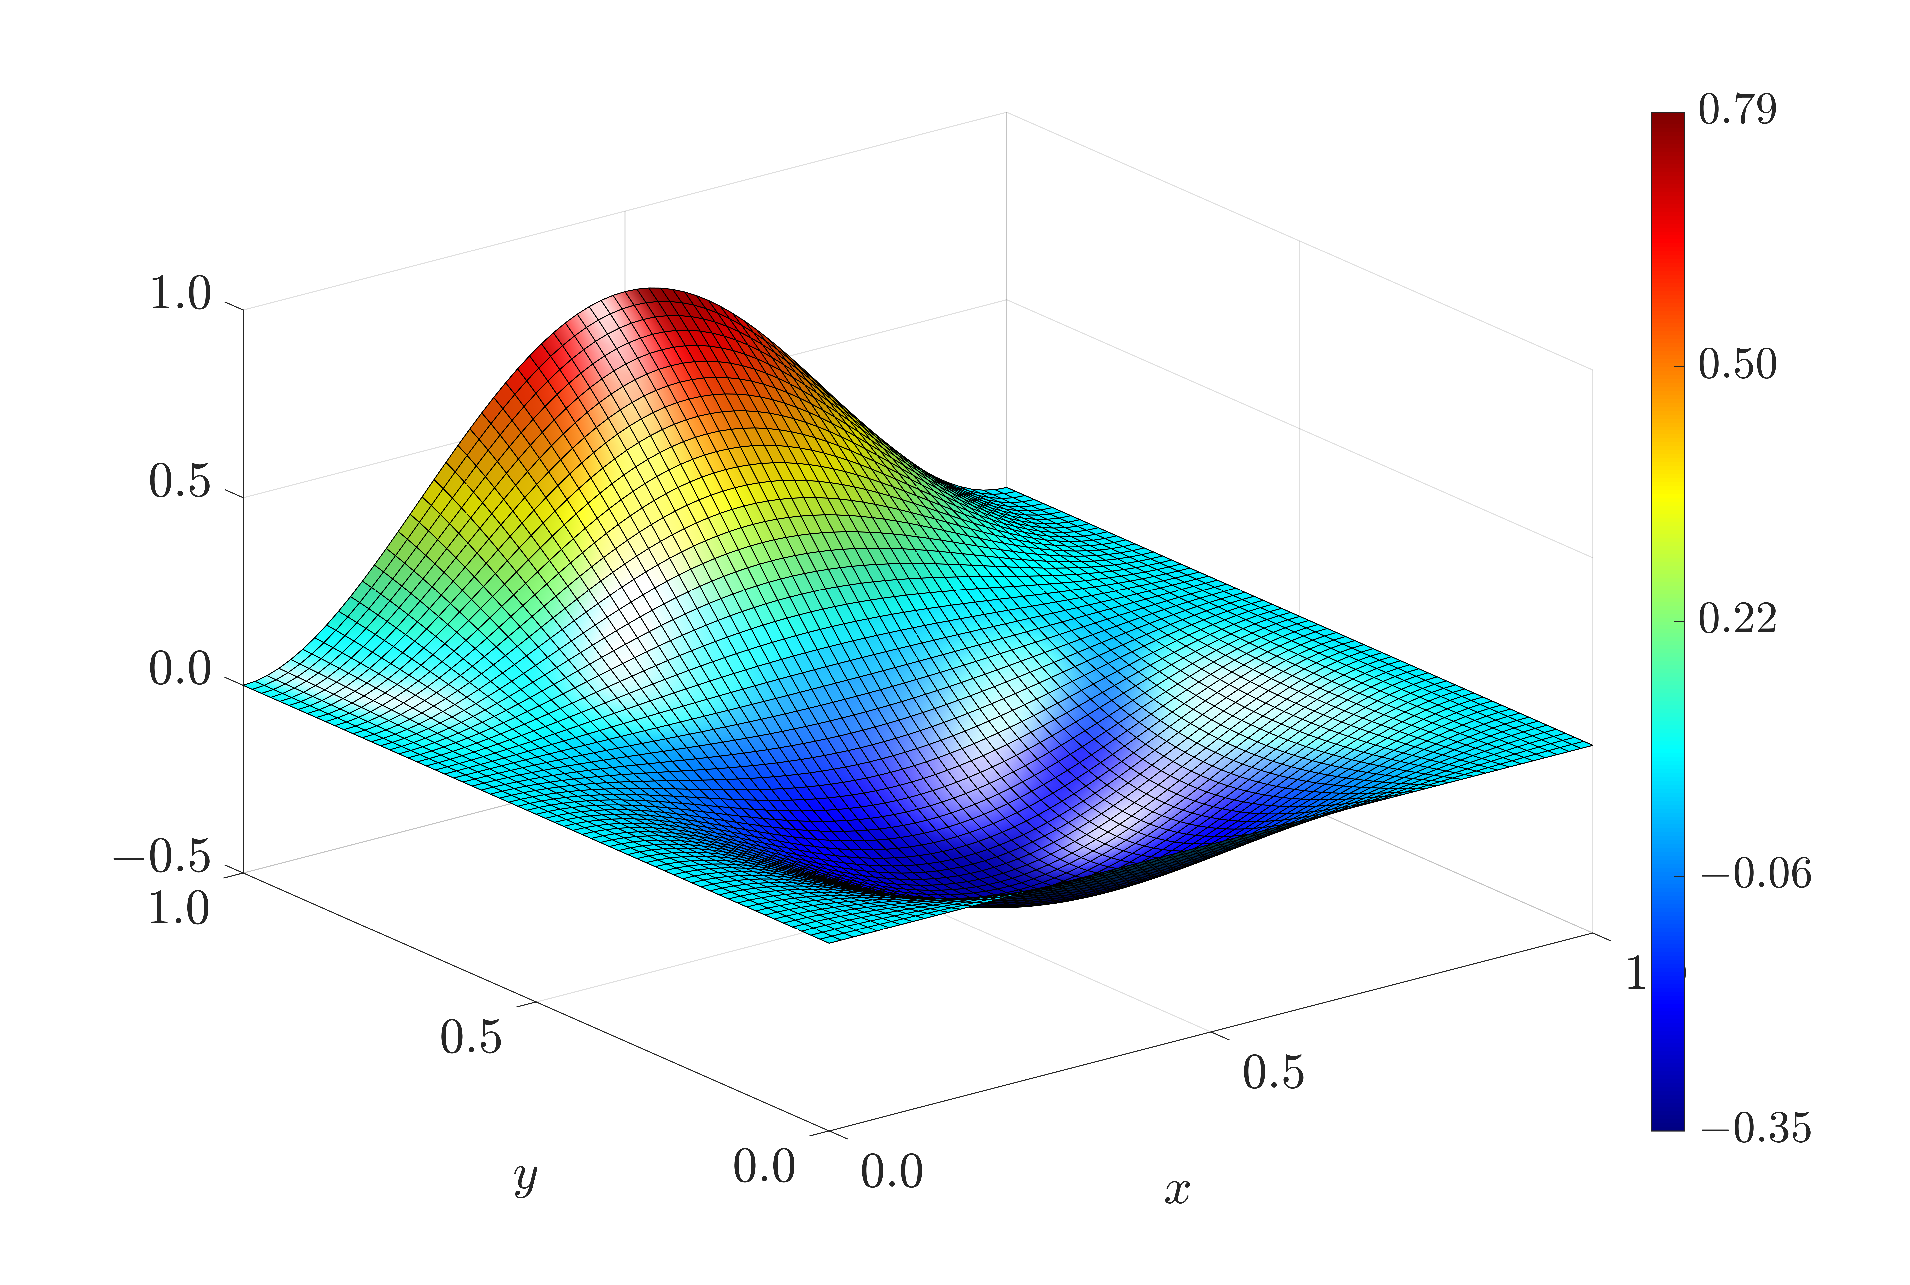
\includegraphics[width=\textwidth]{Figures/Exact_Surf_NormErr_2nd_Betann_0.1_Re_1_Wi_1_epsilon_0_xi_0_alphaG_0_Dt_1e-06_at_0.05_tipsim_1_MMS_12_U.eps}
        \captionof{subfigure}{$\overline{u}$}
        \label{fig_solexauCase1}
    \end{minipage}
    \hfill
    \begin{minipage}{0.48\textwidth}
        \centering
        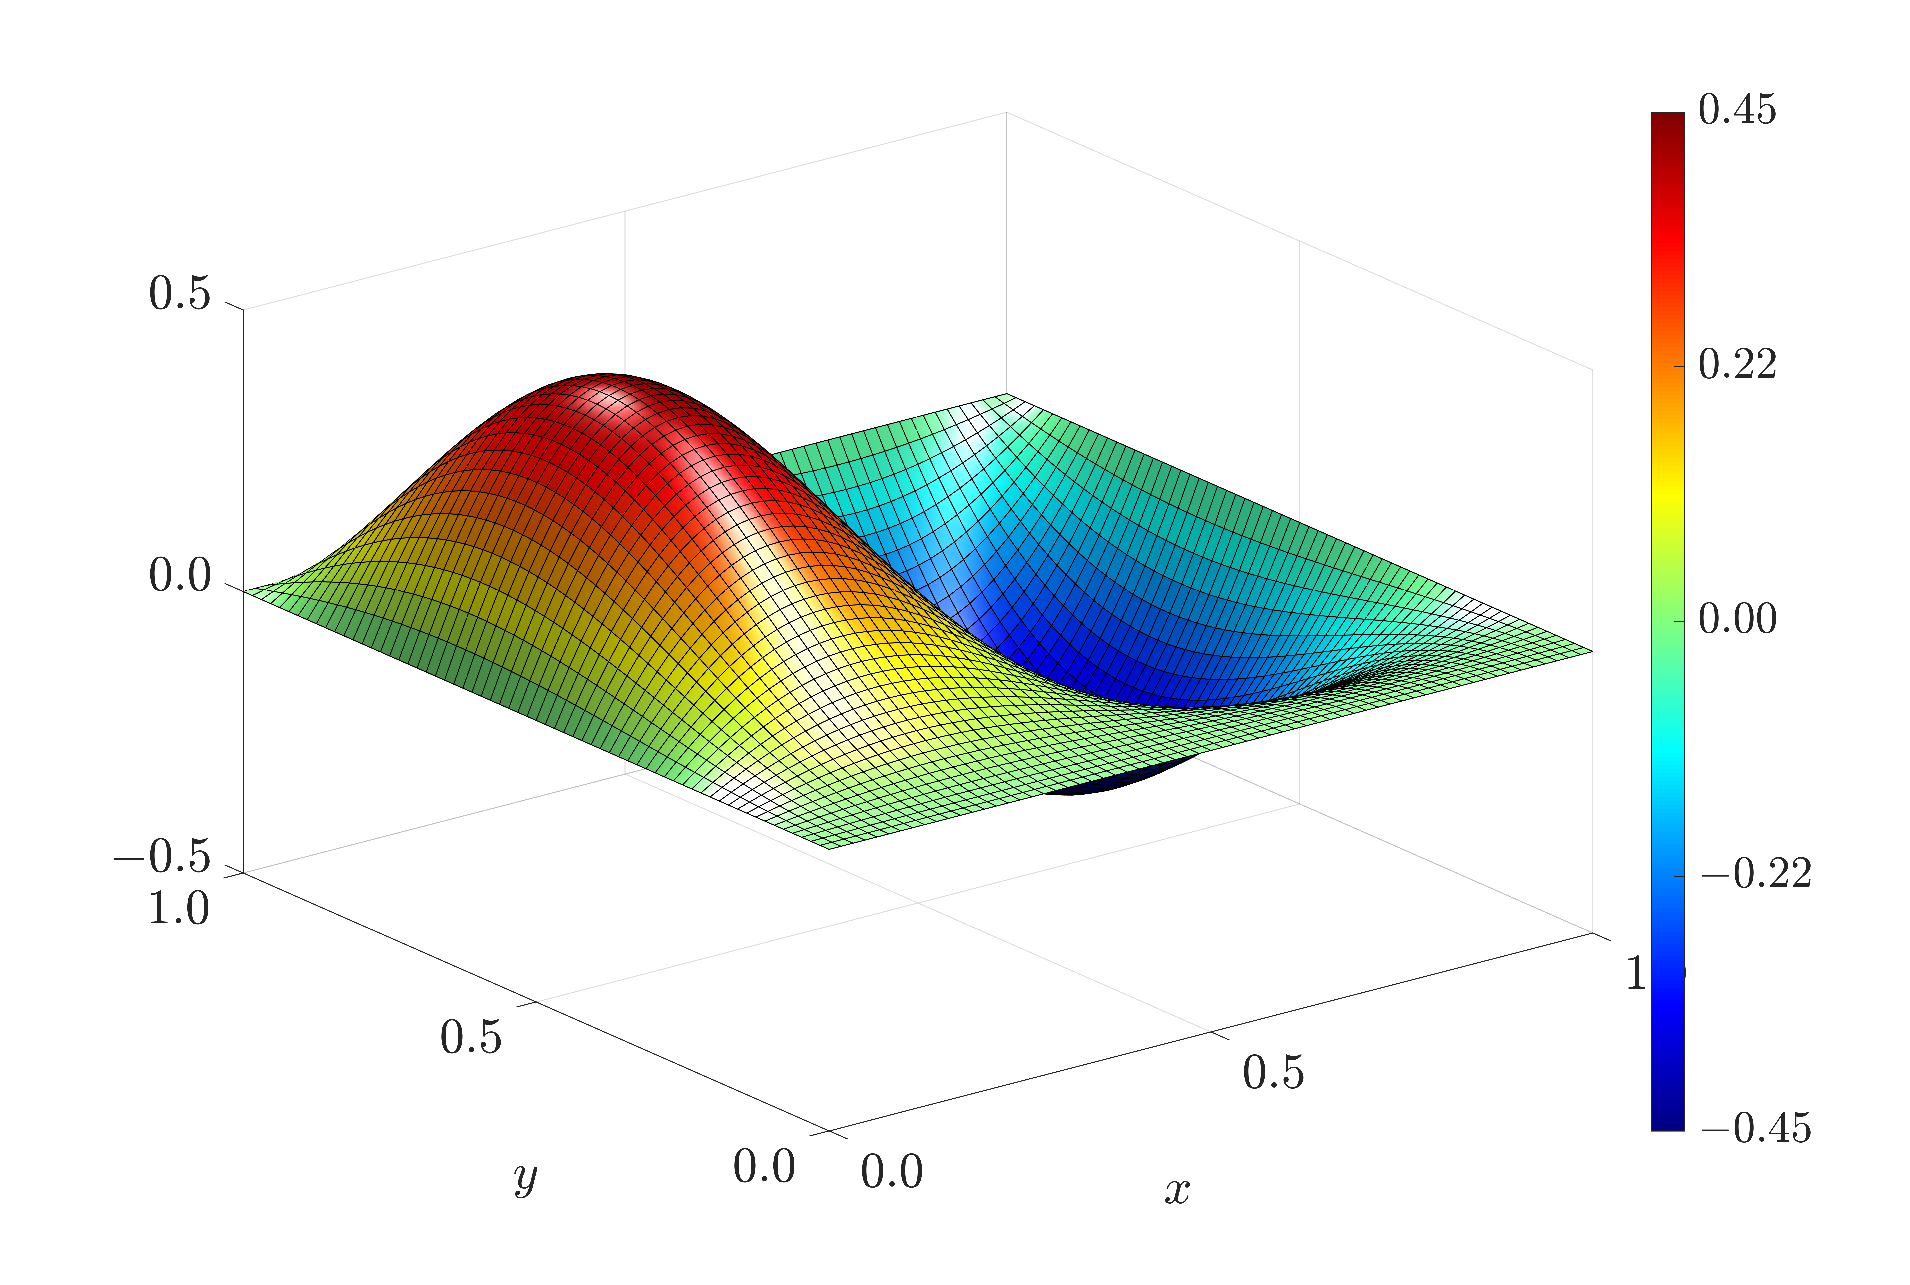
\includegraphics[width=\textwidth]{Figures/Exact_Surf_NormErr_2nd_Betann_0.1_Re_1_Wi_1_epsilon_0_xi_0_alphaG_0_Dt_1e-06_at_0.05_tipsim_1_MMS_12_V.eps}
        \captionof{subfigure}{$\widetilde{v}$}
        \label{fig_solexavCase1}
    \end{minipage}
\end{frame}

%%%%%%%%%%%%%%%%%%%%%%%%%%%%%%%%%%%%%%%%%%%%%%%%%%%%%%%%%%%%%%
\begin{frame}{Soluções Manufaturadas}
    \centering
    \captionsetup{justification=centering}
    \captionof{figure}{Soluções manufaturadas no regime de estado estacionário
    para a vorticidade $(\tilde{\omega_{z}})$ e função de corrente $(\tilde{\psi})$, considerando $a = 0.05$}
    \label{fig:sol_manufaturadas_2}
    \begin{minipage}{0.48\textwidth}
        \centering
        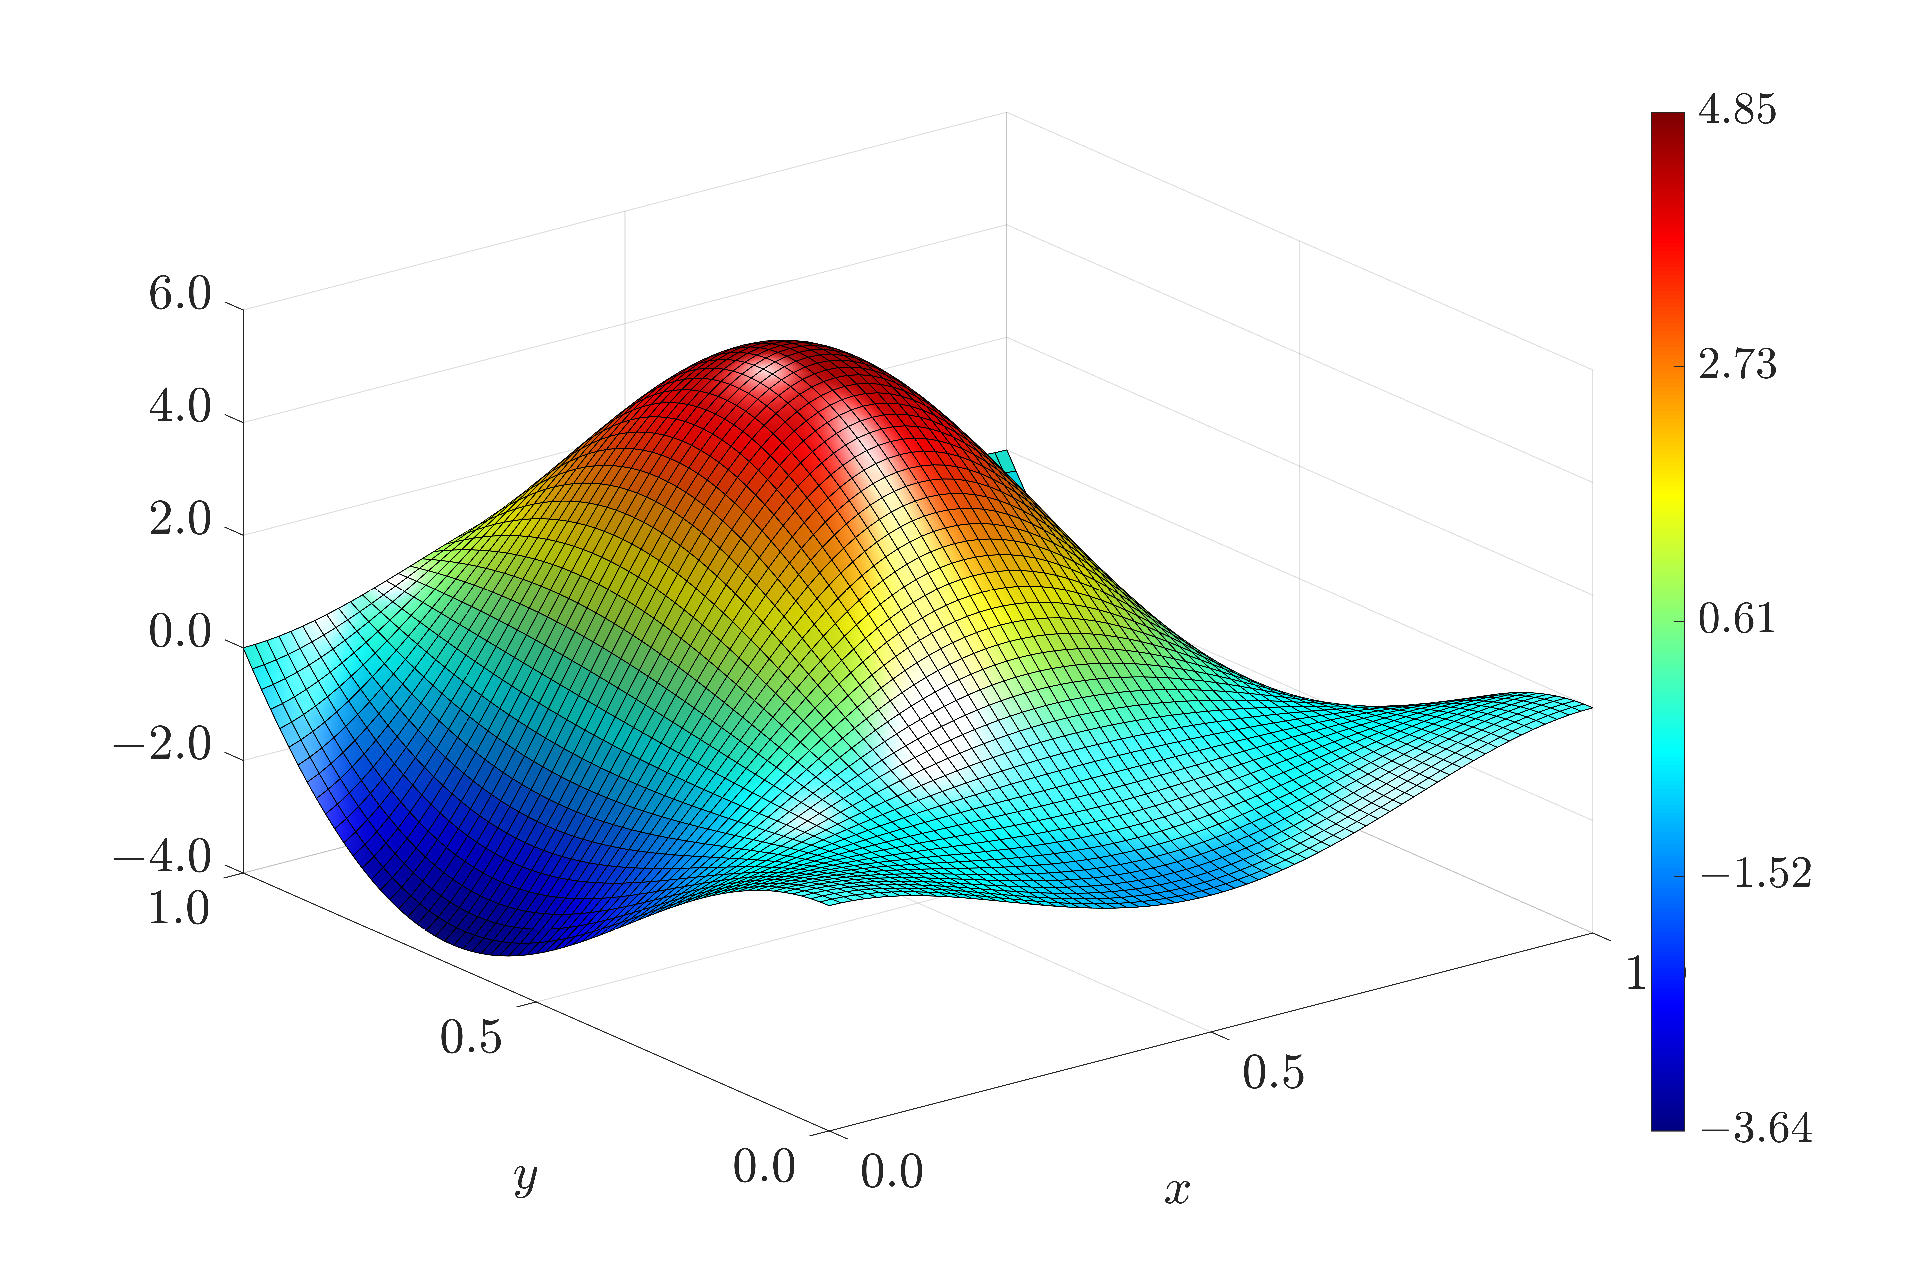
\includegraphics[width=\textwidth]{Figures/Exact_Surf_NormErr_2nd_Betann_0.1_Re_1_Wi_1_epsilon_0_xi_0_alphaG_0_Dt_1e-06_at_0.05_tipsim_1_MMS_12_Wz.eps}
        \captionof{subfigure}{$\widetilde{\omega_{z}}$}
        \label{fig_solexawzCase1}
    \end{minipage}
    \hfill
    \begin{minipage}{0.48\textwidth}
        \centering
        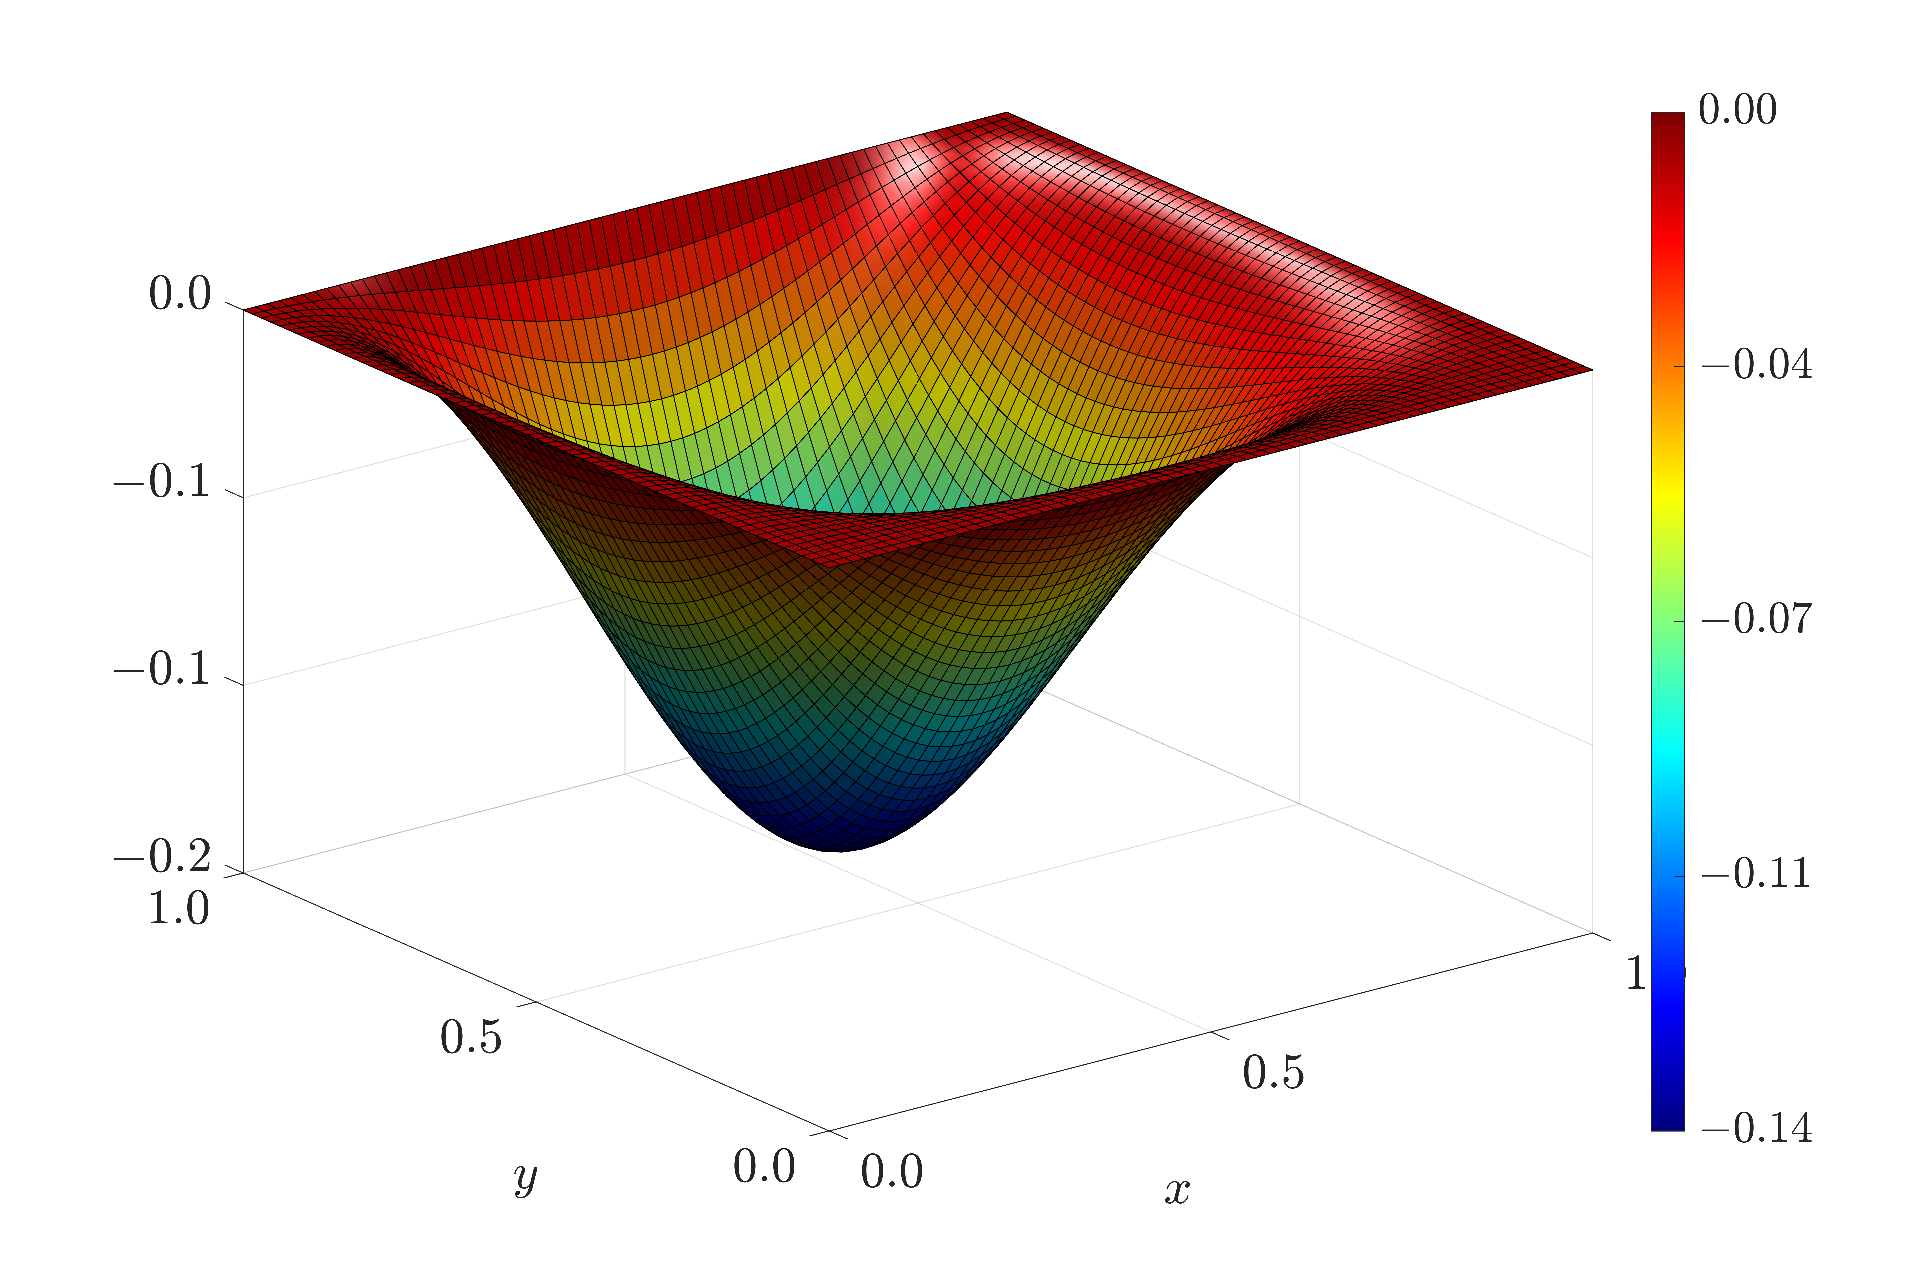
\includegraphics[width=\textwidth]{Figures/Exact_Surf_NormErr_2nd_Betann_0.1_Re_1_Wi_1_epsilon_0_xi_0_alphaG_0_Dt_1e-06_at_0.05_tipsim_1_MMS_12_Psi.eps}
        \captionof{subfigure}{$\widetilde{\psi}$}
        \label{fig_solexapsiCase1}
    \end{minipage}
\end{frame}

%%%%%%%%%%%%%%%%%%%%%%%%%%%%%%%%%%%%%%%%%%%%%%%%%%%%%%%%%%%%%%
\begin{frame}{Soluções Manufaturadas}
    \centering
    \captionsetup{justification=centering}
    \captionof{figure}{Soluções manufaturadas no regime de estado estacionário para os tensores, considerando $\beta_{nn}=0.1$ e $a = 0.05$}
    \label{fig:sol_manufaturadas_3}
    \begin{minipage}{0.31\textwidth}
        \centering
        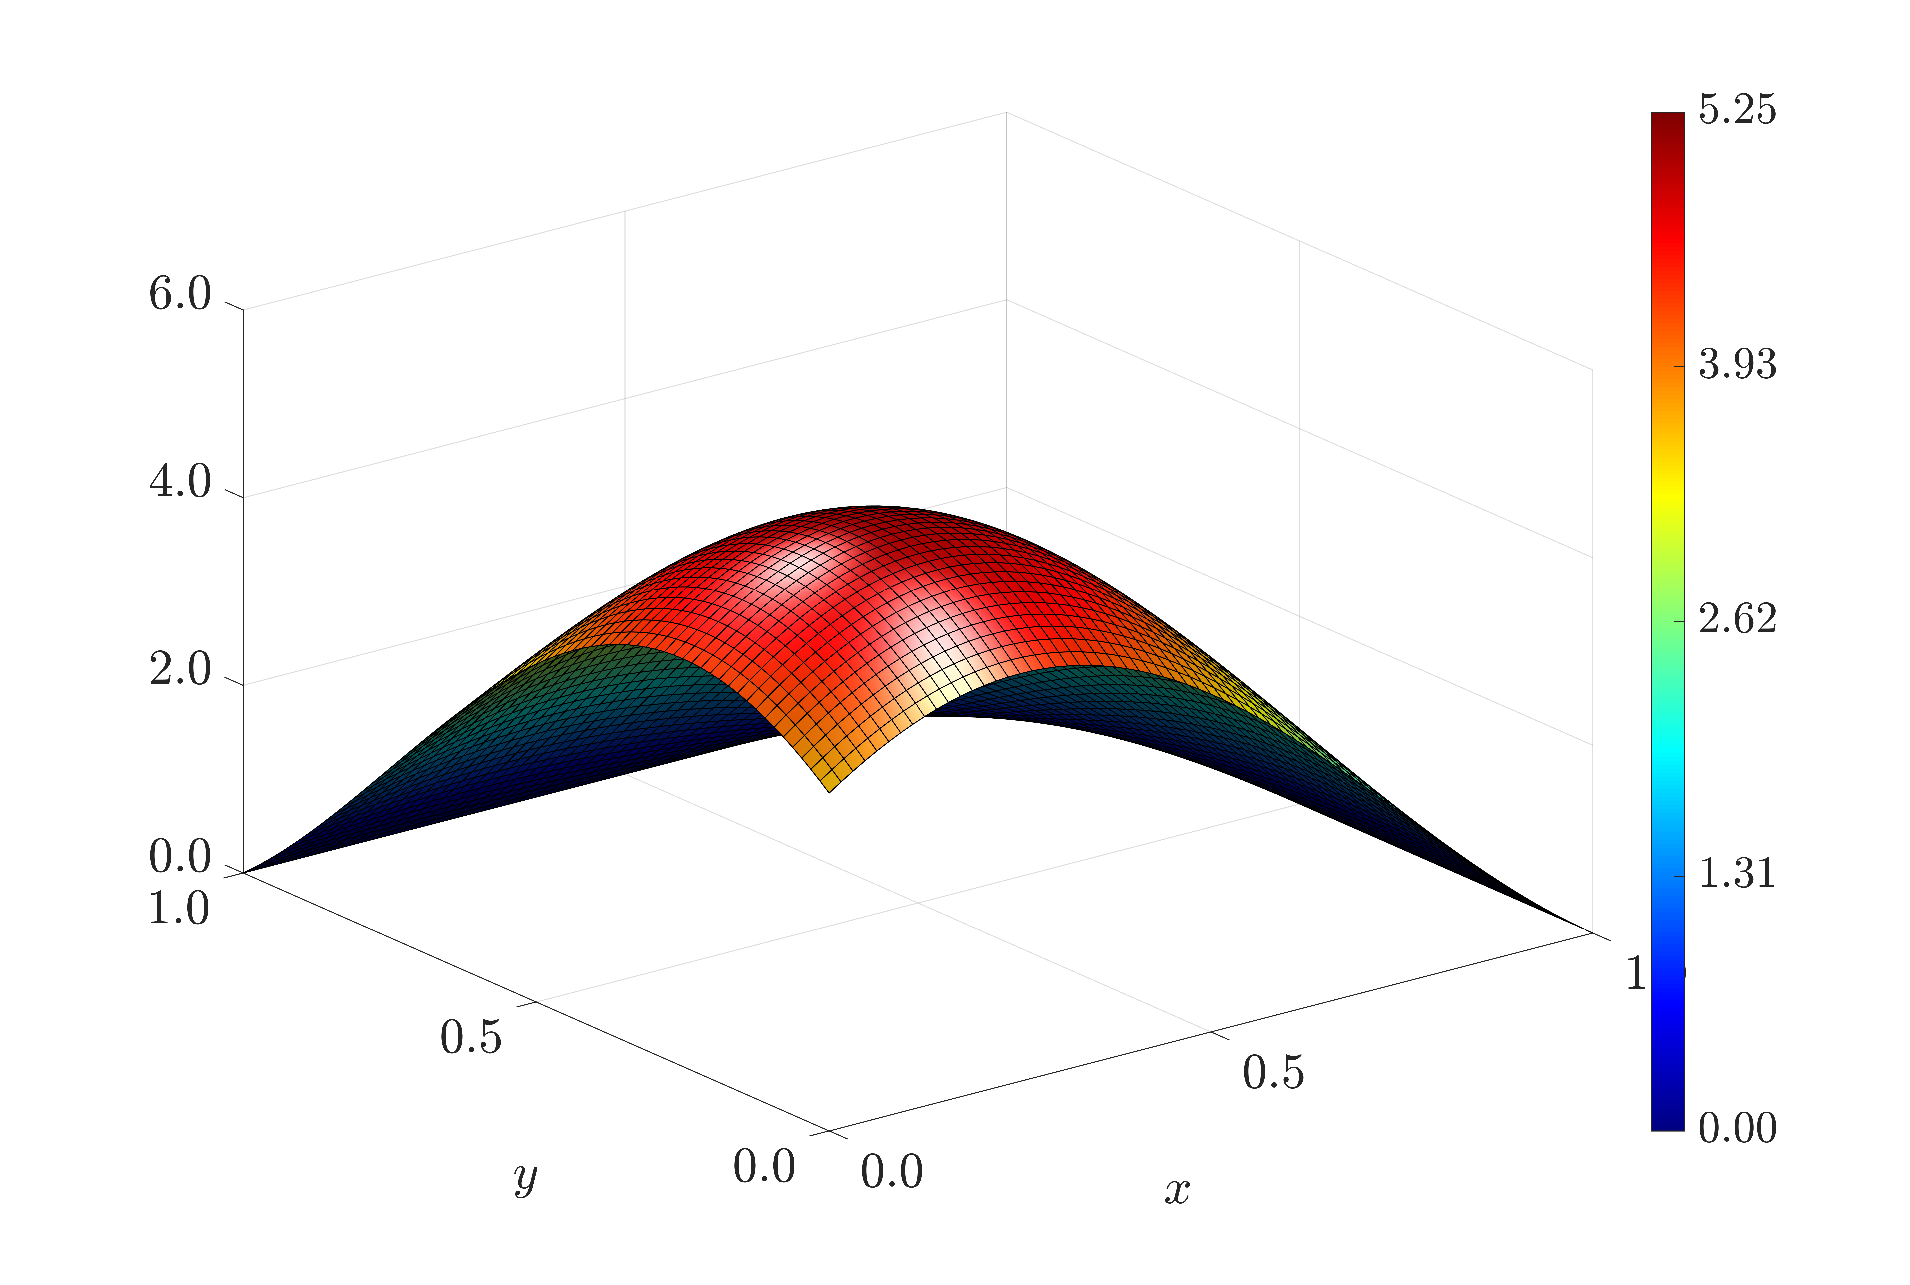
\includegraphics[width=\textwidth]{Figures/Exact_Surf_NormErr_2nd_Betann_0.1_Re_1_Wi_1_epsilon_0_xi_0_alphaG_0_Dt_1e-06_at_0.05_tipsim_1_MMS_12_Txx.eps}
        \captionof{subfigure}{$\overline{T}_{xx}$}
        \label{fig_solexaTxxCase1}
    \end{minipage}
    \hfill
    \begin{minipage}{0.31\textwidth}
        \centering
        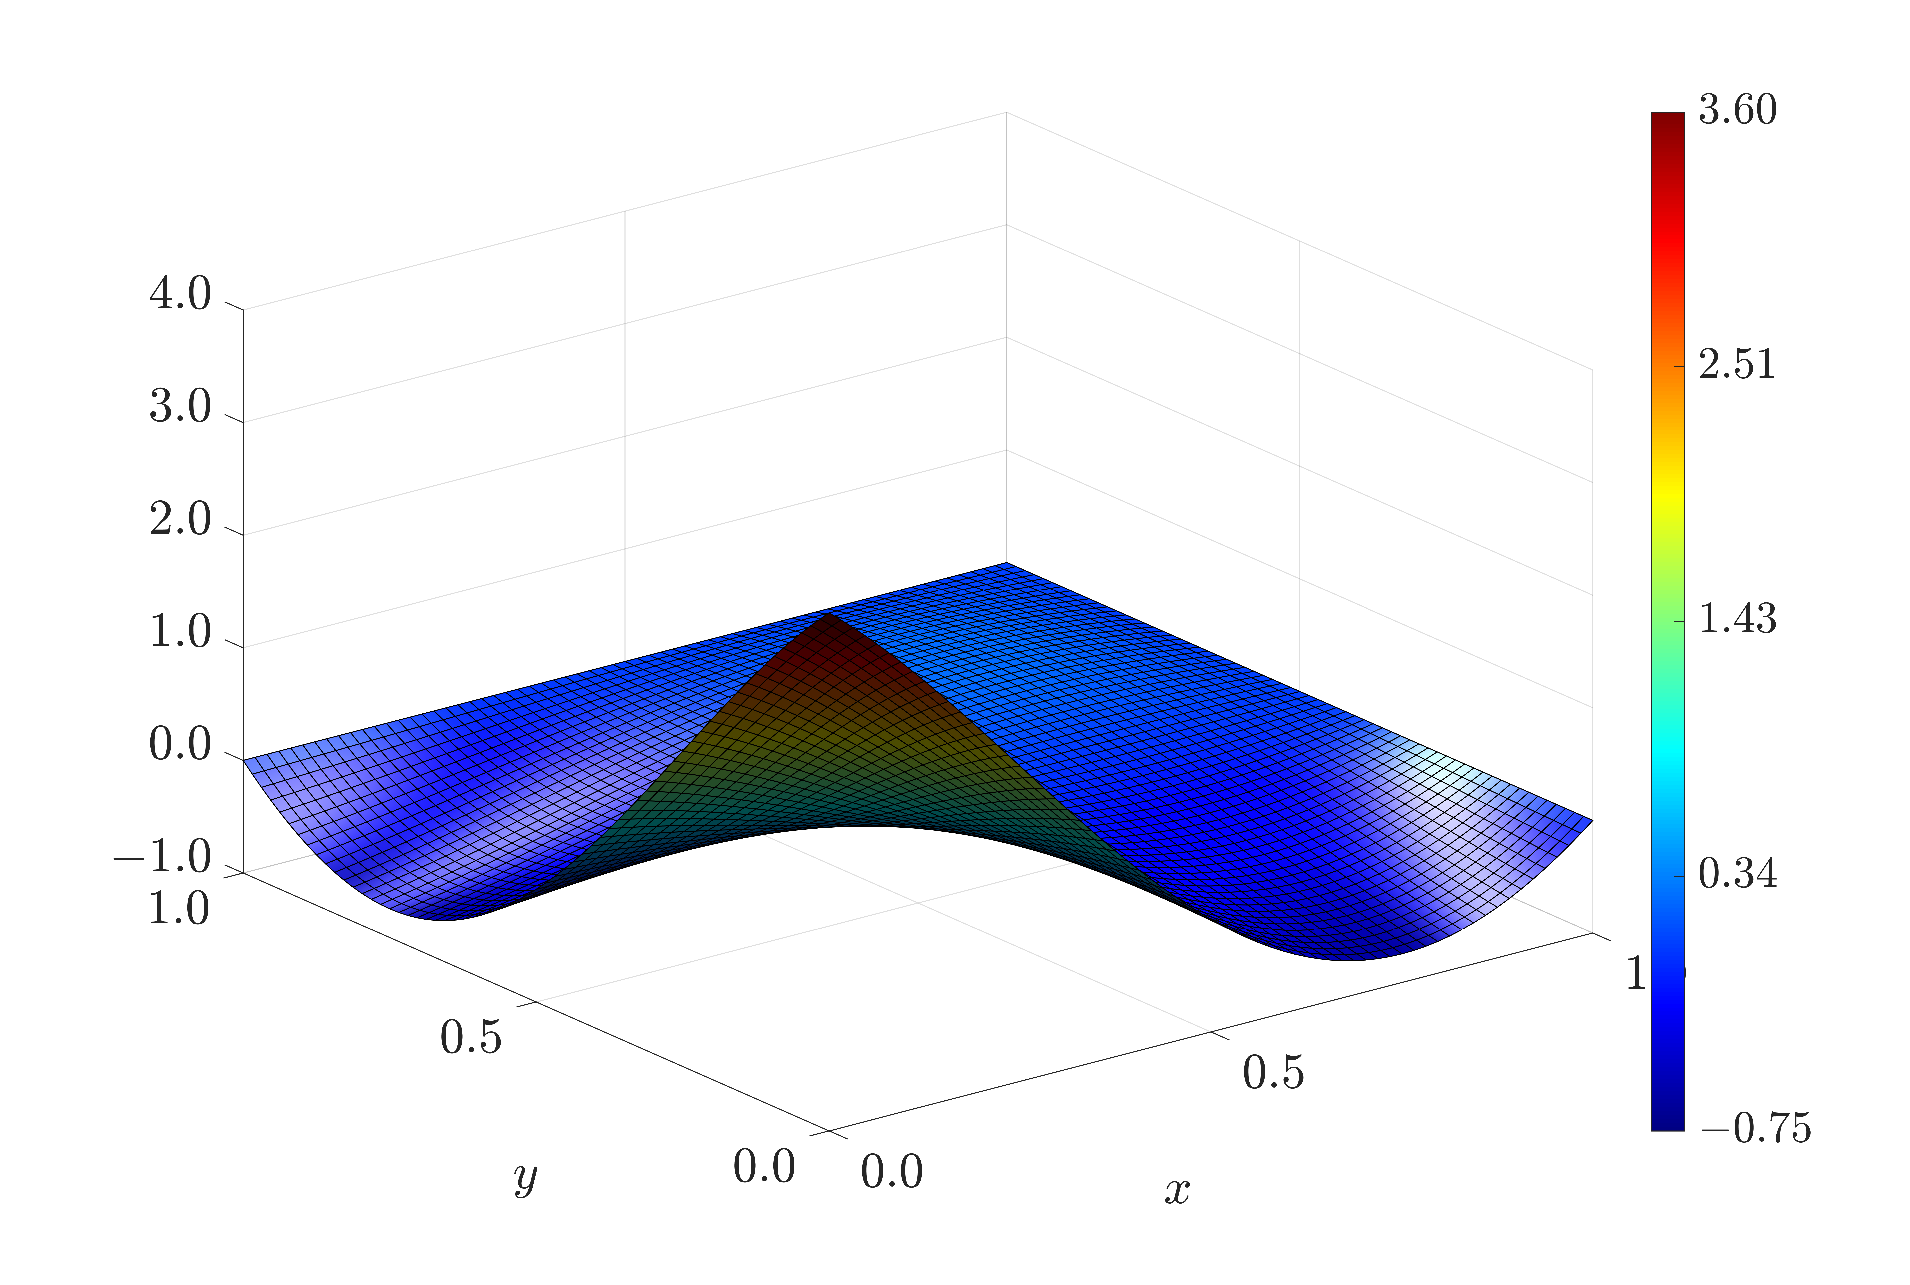
\includegraphics[width=\textwidth]{Figures/Exact_Surf_NormErr_2nd_Betann_0.1_Re_1_Wi_1_epsilon_0_xi_0_alphaG_0_Dt_1e-06_at_0.05_tipsim_1_MMS_12_Txy.eps}
        \captionof{subfigure}{$\overline{T}_{xy}$}
        \label{fig_solexaTxyCase1}
    \end{minipage}
    \hfill
    \begin{minipage}{0.31\textwidth}
        \centering
        \includegraphics[width=\textwidth]{Figures/Exact_Surf_NormErr_2nd_Betann_0.1_Re_1_Wi_1_epsilon_0_xi_0_alphaG_0_Dt_1e-06_at_0.05_tipsim_1_MMS_12_Tyy.eps}
        \captionof{subfigure}{$\overline{T}_{yy}$}
        \label{fig_solexaTyyCase1}
    \end{minipage}
\end{frame}


%%%%%%%%%%%%%%%%%%%%%%%%%%%%%%%%%%%%%%%%%%%%%%%%%%%%%%%%%%%%%%
\begin{frame}{Soluções Manufaturadas}
    \centering
    \captionsetup{justification=centering}
    \captionof{figure}{Soluções manufaturadas no regime de estado estacionário para o campo de velocidades $(\overline{u},\tilde{v})$, considerando $a = 0.05$}
    \label{fig:sol_manufaturadas_11}
    \begin{minipage}{0.48\textwidth}
        \centering
        \includegraphics[width=\textwidth]{Figures/Exact_Map_NormErr_2nd_Betann_0.1_Re_1_Wi_1_epsilon_0_xi_0_alphaG_0_Dt_1e-06_at_0.05_tipsim_1_MMS_12_U.eps}
        \captionof{subfigure}{$\overline{u}$}
        \label{fig_solexauCase11}
    \end{minipage}
    \hfill
    \begin{minipage}{0.48\textwidth}
        \centering
        \includegraphics[width=\textwidth]{Figures/Exact_Map_NormErr_2nd_Betann_0.1_Re_1_Wi_1_epsilon_0_xi_0_alphaG_0_Dt_1e-06_at_0.05_tipsim_1_MMS_12_V.eps}
        \captionof{subfigure}{$\widetilde{v}$}
        \label{fig_solexavCase11}
    \end{minipage}
\end{frame}

%%%%%%%%%%%%%%%%%%%%%%%%%%%%%%%%%%%%%%%%%%%%%%%%%%%%%%%%%%%%%%
\begin{frame}{Soluções Manufaturadas}
    \centering
    \captionsetup{justification=centering}
    \captionof{figure}{Soluções manufaturadas no regime de estado estacionário
    para a vorticidade $(\tilde{\omega_{z}})$ e função de corrente $(\tilde{\psi})$, considerando $a = 0.05$}
    \label{fig:sol_manufaturadas_21}
    \begin{minipage}{0.48\textwidth}
        \centering
        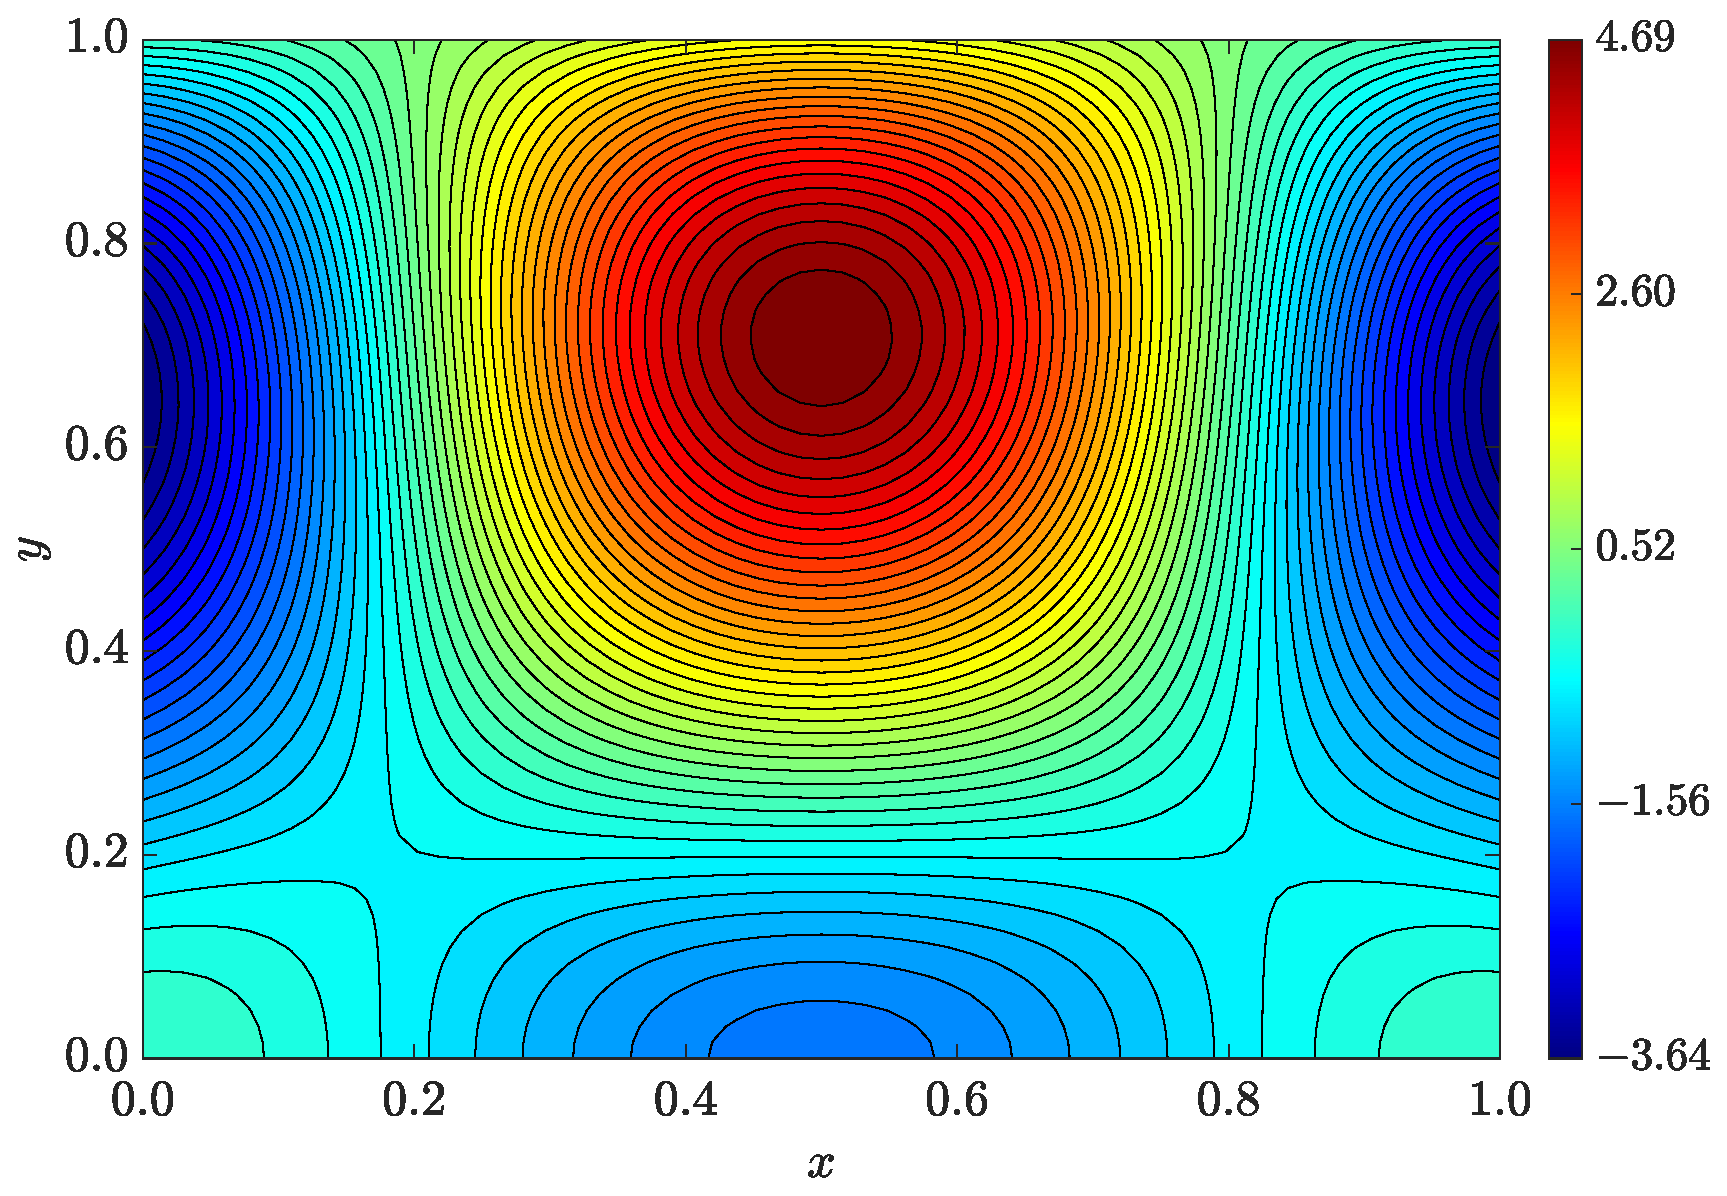
\includegraphics[width=\textwidth]{Figures/Exact_Map_NormErr_2nd_Betann_0.1_Re_1_Wi_1_epsilon_0_xi_0_alphaG_0_Dt_1e-06_at_0.05_tipsim_1_MMS_12_Wz.eps}
        \captionof{subfigure}{$\widetilde{\omega_{z}}$}
        \label{fig_solexawzCase11}
    \end{minipage}
    \hfill
    \begin{minipage}{0.48\textwidth}
        \centering
        \includegraphics[width=\textwidth]{Figures/Exact_Map_NormErr_2nd_Betann_0.1_Re_1_Wi_1_epsilon_0_xi_0_alphaG_0_Dt_1e-06_at_0.05_tipsim_1_MMS_12_Psi.eps}
        \captionof{subfigure}{$\widetilde{\psi}$}
        \label{fig_solexapsiCase11}
    \end{minipage}
\end{frame}

%%%%%%%%%%%%%%%%%%%%%%%%%%%%%%%%%%%%%%%%%%%%%%%%%%%%%%%%%%%%%%
\begin{frame}{Soluções Manufaturadas}
    \centering
    \captionsetup{justification=centering}
    \captionof{figure}{Soluções manufaturadas no regime de estado estacionário para os tensores, considerando $\beta_{nn}=0.1$ e $a = 0.05$}
    \label{fig:sol_manufaturadas_31}
    \begin{minipage}{0.31\textwidth}
        \centering
        \includegraphics[width=\textwidth]{Figures/Exact_Map_NormErr_2nd_Betann_0.1_Re_1_Wi_1_epsilon_0_xi_0_alphaG_0_Dt_1e-06_at_0.05_tipsim_1_MMS_12_Txx.eps}
        \captionof{subfigure}{$\overline{T}_{xx}$}
        \label{fig_solexaTxxCase11}
    \end{minipage}
    \hfill
    \begin{minipage}{0.31\textwidth}
        \centering
        \includegraphics[width=\textwidth]{Figures/Exact_Map_NormErr_2nd_Betann_0.1_Re_1_Wi_1_epsilon_0_xi_0_alphaG_0_Dt_1e-06_at_0.05_tipsim_1_MMS_12_Txy.eps}
        \captionof{subfigure}{$\overline{T}_{xy}$}
        \label{fig_solexaTxyCase11}
    \end{minipage}
    \hfill
    \begin{minipage}{0.31\textwidth}
        \centering
        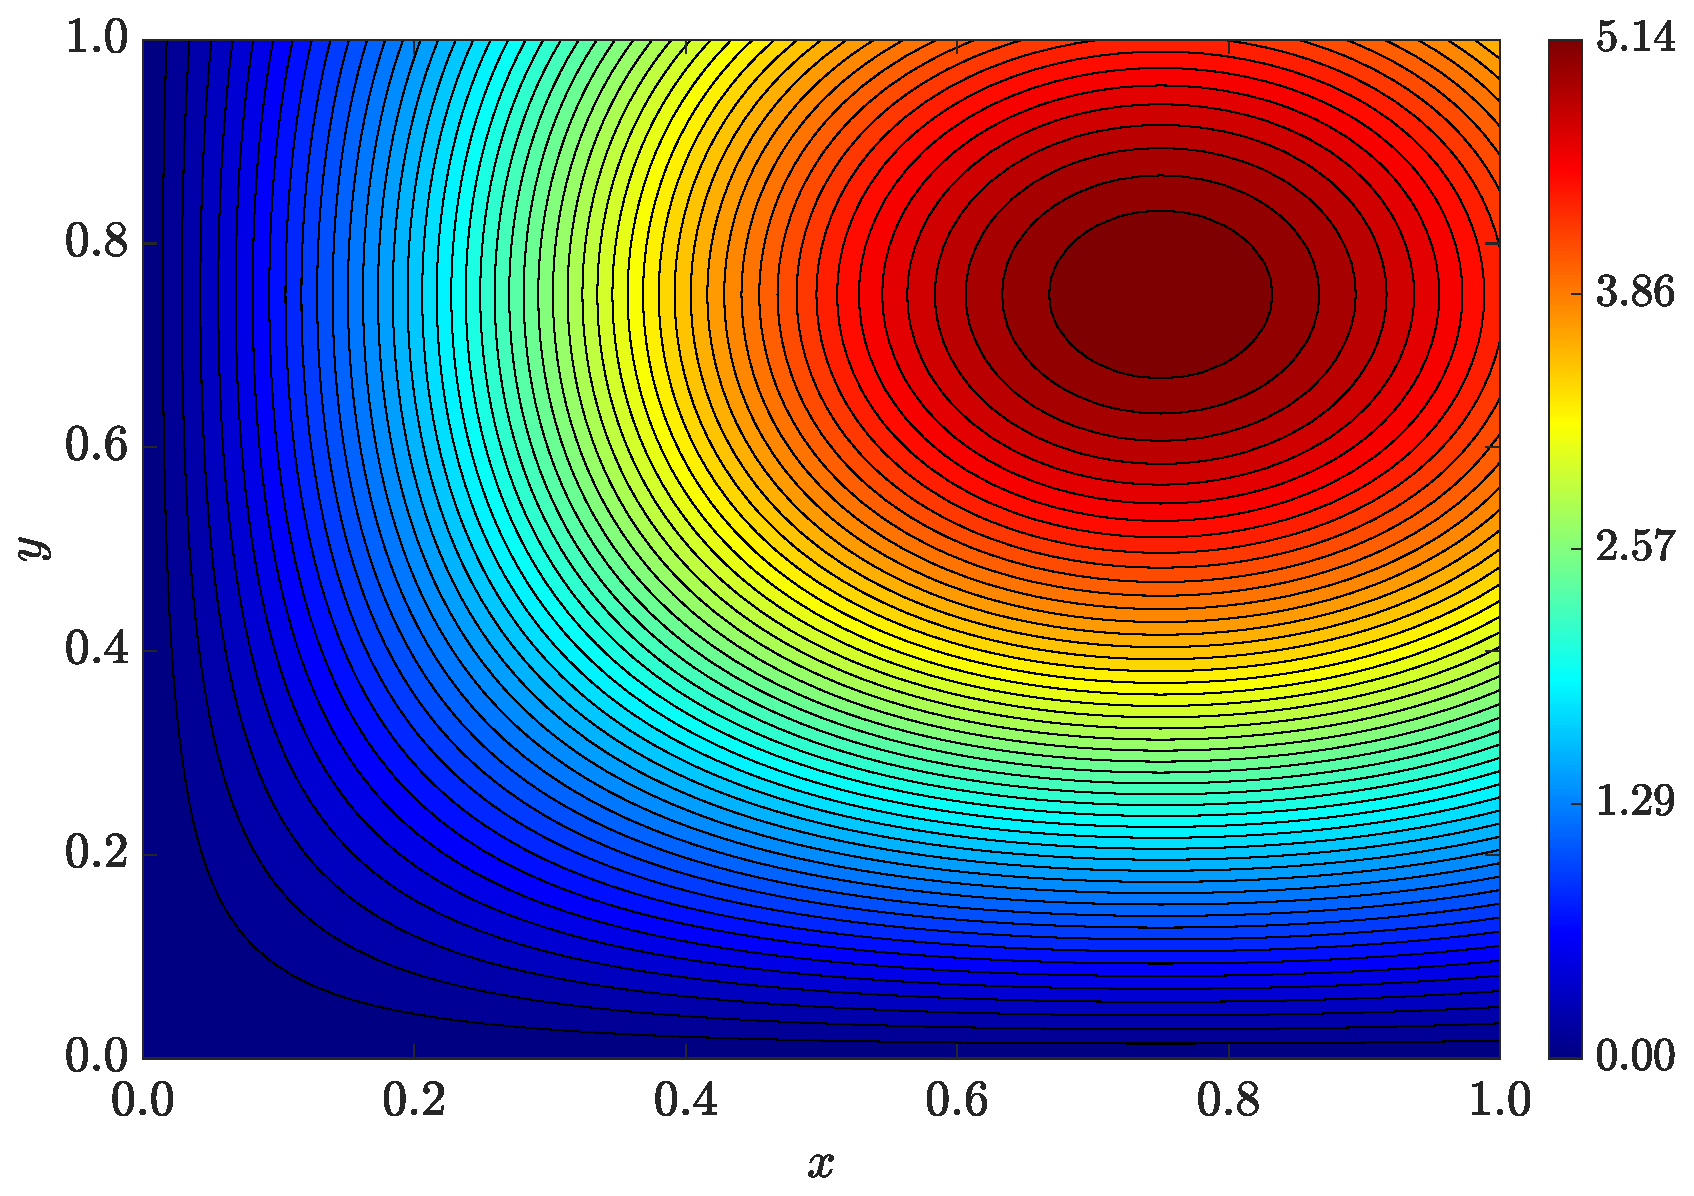
\includegraphics[width=\textwidth]{Figures/Exact_Map_NormErr_2nd_Betann_0.1_Re_1_Wi_1_epsilon_0_xi_0_alphaG_0_Dt_1e-06_at_0.05_tipsim_1_MMS_12_Tyy.eps}
        \captionof{subfigure}{$\overline{T}_{yy}$}
        \label{fig_solexaTyyCase11}
    \end{minipage}
\end{frame}

%%%%%%%%%%%%%%%%%%%%%%%%%%%%%%%%%%%%%%%%%%%%%%%%%%%%%%%%%%%%%%
\begin{frame}{Soluções Manufaturadas}
    \centering
    \captionsetup{justification=centering}
    \captionof{figure}{Soluções manufaturadas no regime de estado estacionário para os tensores, considerando $\beta_{nn}=0.1$ e $a = 0.05$}
    \label{fig:sol_manufaturadas_311}
    \begin{minipage}{0.31\textwidth}
        \centering
        \includegraphics[width=\textwidth]{Figures/Exact_Map_NormErr_2nd_Betann_0.1_Re_1_Wi_1_epsilon_0_xi_0_alphaG_0_Dt_1e-06_at_0.05_tipsim_1_MMS_12_Txx.eps}
        \captionof{subfigure}{$\overline{T}_{xx}$}
        \label{fig_solexaTxxCase111}
    \end{minipage}
    \hfill
    \begin{minipage}{0.31\textwidth}
        \centering
        \includegraphics[width=\textwidth]{Figures/Exact_Map_NormErr_2nd_Betann_0.1_Re_1_Wi_1_epsilon_0_xi_0_alphaG_0_Dt_1e-06_at_0.05_tipsim_1_MMS_12_Txy.eps}
        \captionof{subfigure}{$\overline{T}_{xy}$}
        \label{fig_solexaTxyCase111}
    \end{minipage}
    \hfill
    \begin{minipage}{0.31\textwidth}
        \centering
        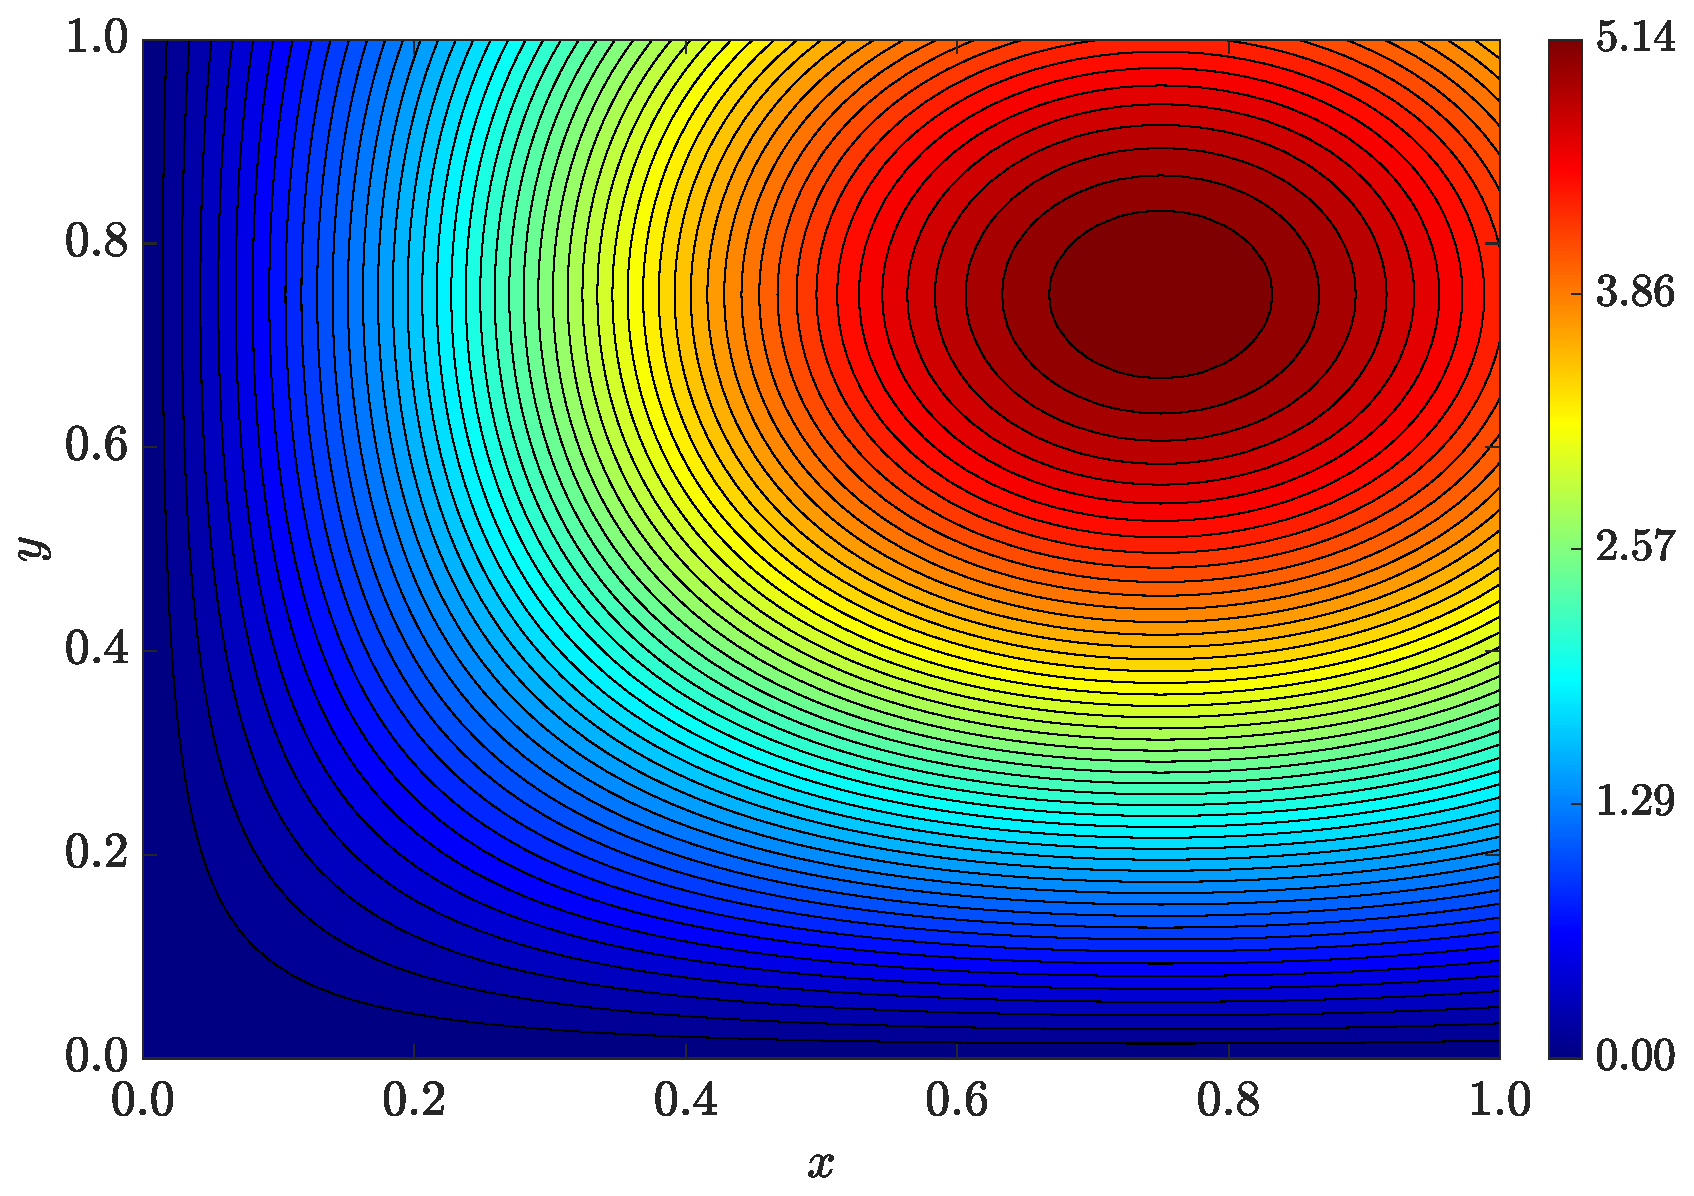
\includegraphics[width=\textwidth]{Figures/Exact_Map_NormErr_2nd_Betann_0.1_Re_1_Wi_1_epsilon_0_xi_0_alphaG_0_Dt_1e-06_at_0.05_tipsim_1_MMS_12_Tyy.eps}
        \captionof{subfigure}{$\overline{T}_{yy}$}
        \label{fig_solexaTyyCase111}
    \end{minipage}
\end{frame}

%%%%%%%%%%%%%%%%%%%%%%%%%%%%%%%%%%%%%%%%%%%%%%%%%%%%%%%%%%%%%%
\begin{frame}{Caso de verificação usando o modelo UCM}
    \centering
    \begin{table}[H]
    \caption{Erros numéricos e cálculo da ordem de convergência para a vorticidade $(\omega_{z})$, utilizando o parâmetro $Wi=1$, para o escoamento de fluido viscoelástico UCM.\label{tab_UCMWzResumida_1}}
\scriptsize{
    \begin{minipage}{0.49\textwidth}
    \begin{tabular*}{\textwidth}{@{\extracolsep\fill}cccc@{}}
    \hline
    \multirow{2}{*}{$\operatorname{Re}$} & \multirow{2}{*}{Malha} & \multicolumn{2}{c}{$\beta_{nn}=0.0$}\\ %\cline{2-10}
     & & Erro & Ordem \\
    \hline
    \multirow{7}{*}{1.00} & $17\times 17$ & 3.10e-03 & --- \\
    & $33\times 33$ & 2.93e-04 & 3.40 \\
    & $49\times 49$ & 6.78e-05 & 3.61 \\
    & $65\times 65$ & 2.31e-05 & 3.74 \\
    & $81\times 81$ & 9.80e-06 & 3.85 \\
    & $97\times 97$ & 4.72e-06 & 4.01 \\
    & $113\times 113$ & 2.46e-06 & 4.22 \\
    & $129\times 129$ & 1.41e-06 & 4.16 \\
    \hline
    \multirow{7}{*}{100.00} & $17\times 17$ & 3.10e-03 & --- \\
    & $33\times 33$ & 2.93e-04 & 3.40 \\
    & $49\times 49$ & 6.78e-05 & 3.61 \\
    & $65\times 65$ & 2.32e-05 & 3.74 \\
    & $81\times 81$ & 9.83e-06 & 3.84 \\
    & $97\times 97$ & 4.74e-06 & 4.00 \\
    & $113\times 113$ & 2.48e-06 & 4.21 \\
    & $129\times 129$ & 1.42e-06 & 4.16 \\
    \hline
    \end{tabular*}
    \end{minipage}
    \hfill
    \begin{minipage}{0.49\textwidth}
    \begin{tabular*}{\textwidth}{@{\extracolsep\fill}cccc@{}}
    \hline
    \multirow{2}{*}{$\operatorname{Re}$} & \multirow{2}{*}{Malha} & \multicolumn{2}{c}{$\beta_{nn}=0.0$}\\
     & & Erro & Ordem \\
    \hline
    \multirow{7}{*}{400.00} & $17\times 17$ & 3.10e-03 & --- \\
    & $33\times 33$ & 2.93e-04 & 3.40 \\
    & $49\times 49$ & 6.78e-05 & 3.61 \\
    & $65\times 65$ & 2.32e-05 & 3.74 \\
    & $81\times 81$ & 9.83e-06 & 3.84 \\
    & $97\times 97$ & 4.74e-06 & 4.00 \\
    & $113\times 113$ & 2.48e-06 & 4.21 \\
    & $129\times 129$ & 1.42e-06 & 4.16 \\
    \hline
    \multirow{7}{*}{1000.00} & $17\times 17$ & 3.10e-03 & --- \\
    & $33\times 33$ & 2.93e-04 & 3.40 \\
    & $49\times 49$ & 6.78e-05 & 3.61 \\
    & $65\times 65$ & 2.32e-05 & 3.74 \\
    & $81\times 81$ & 9.83e-06 & 3.84 \\
    & $97\times 97$ & 4.74e-06 & 4.00 \\
    & $113\times 113$ & 2.48e-06 & 4.21 \\
    & $129\times 129$ & 1.42e-06 & 4.16 \\
    \hline
    \end{tabular*}
    \end{minipage}
}
\end{table}
\end{frame}

%%%%%%%%%%%%%%%%%%%%%%%%%%%%%%%%%%%%%%%%%%%%%%%%%%%%%%%%%%%%%%
\begin{frame}{Caso de verificação usando o modelo UCM}
    \centering
    \captionsetup{justification=centering}
    \captionof{figure}{Erro para o campo de velocidades $(\overline{u},\tilde{v})$ utilizando $Re=100$, $\beta_{nn} = 0$ e $Wi=1$ para o escoamento de fluido viscoelástico como o modelo UCM}
    \label{fig:ucm_1}
    \begin{minipage}{0.49\textwidth}
        \centering
        \includegraphics[width=\textwidth]{Figures/UCM/NormErr_2nd_Re_100_Wi_1_epsilon_0_xi_0_alphaG_0_Dt_1e-06_at_0.05_tipsim_1_MMS_12_U.eps}
        \captionof{subfigure}{$\overline{u}$}
        \label{ucm_u_Case11}
    \end{minipage}
    \hfill
    \begin{minipage}{0.49\textwidth}
        \centering
        \includegraphics[width=\textwidth]{Figures/UCM/NormErr_2nd_Re_100_Wi_1_epsilon_0_xi_0_alphaG_0_Dt_1e-06_at_0.05_tipsim_1_MMS_12_V.eps}
        \captionof{subfigure}{$\tilde{v}$}
        \label{ucm_v_Case11}
    \end{minipage}
\end{frame}

%%%%%%%%%%%%%%%%%%%%%%%%%%%%%%%%%%%%%%%%%%%%%%%%%%%%%%%%%%%%%%
\begin{frame}{Caso de verificação usando o modelo UCM}
    \centering
    \captionsetup{justification=centering}
    \captionof{figure}{Erro para a vorticidade $(\tilde{\omega_{z}})$ e função de corrente $(\tilde{\psi})$, utilizando $Re=100$, $\beta_{nn} = 0$ e $Wi=1$ para o escoamento de fluido viscoelástico como o modelo UCM}
    \label{fig:ucm_2}
    \begin{minipage}{0.49\textwidth}
        \centering
        \includegraphics[width=\textwidth]{Figures/UCM/NormErr_2nd_Re_100_Wi_1_epsilon_0_xi_0_alphaG_0_Dt_1e-06_at_0.05_tipsim_1_MMS_12_Wz.eps}
        \captionof{subfigure}{$\tilde{\omega_{z}}$}
        \label{ucm_wz_Case11}
    \end{minipage}
    \hfill
    \begin{minipage}{0.49\textwidth}
        \centering
        \includegraphics[width=\textwidth]{Figures/UCM/NormErr_2nd_Re_100_Wi_1_epsilon_0_xi_0_alphaG_0_Dt_1e-06_at_0.05_tipsim_1_MMS_12_Psi.eps}
        \captionof{subfigure}{$\tilde{\psi}$}
        \label{ucm_psi_Case11}
    \end{minipage}
\end{frame}

%%%%%%%%%%%%%%%%%%%%%%%%%%%%%%%%%%%%%%%%%%%%%%%%%%%%%%%%%%%%%%
\begin{frame}{Caso de verificação usando o modelo UCM}
    \centering
    \captionsetup{justification=centering}
    \captionof{figure}{Erro para as componentes dos tensores de tensões, utilizando $Re=100$, $\beta_{nn} = 0$ e $Wi=1$ para o escoamento de fluido viscoelástico como o modelo UCM}
    \label{fig:ucm_3}
    \begin{minipage}{0.325\textwidth}
        \centering
        \includegraphics[width=\textwidth]{Figures/UCM/NormErr_2nd_Re_100_Wi_1_epsilon_0_xi_0_alphaG_0_Dt_1e-06_at_0.05_tipsim_1_MMS_12_Txx.eps}
        \captionof{subfigure}{$\overline{T_{xx}}$}
        \label{ucm_txx_Case11}
    \end{minipage}
    \hfill
    \begin{minipage}{0.325\textwidth}
        \centering
        \includegraphics[width=\textwidth]{Figures/UCM/NormErr_2nd_Re_100_Wi_1_epsilon_0_xi_0_alphaG_0_Dt_1e-06_at_0.05_tipsim_1_MMS_12_Txy.eps}
        \captionof{subfigure}{$\overline{T_{xy}}$}
        \label{ucm_txy_Case11}
    \end{minipage}
    \hfill
    \begin{minipage}{0.325\textwidth}
        \centering
        \includegraphics[width=\textwidth]{Figures/UCM/NormErr_2nd_Re_100_Wi_1_epsilon_0_xi_0_alphaG_0_Dt_1e-06_at_0.05_tipsim_1_MMS_12_Tyy.eps}
        \captionof{subfigure}{$\overline{T_{yy}}$}
        \label{ucm_tyy_Case11}
    \end{minipage}
\end{frame}

%%%%%%%%%%%%%%%%%%%%%%%%%%%%%%%%%%%%%%%%%%%%%%%%%%%%%%%%%%%%%%
\begin{frame}{Caso de verificação usando o modelo Oldroyd-B}
    \centering
    \begin{table}[H]
\caption{Erros numéricos e cálculo da ordem de convergência para a vorticidade $(\omega_{z})$, utilizando o parâmetro $Wi=1$, para o escoamento de fluido viscoelástico Oldroyd-B.\label{tab_OldroydBWzResumida}}
\scriptsize{
    \begin{tabular*}{\textwidth}{@{\extracolsep\fill}cccccccccc@{}}
    \hline
    \multirow{2}{*}{$\operatorname{Re}$} & \multirow{2}{*}{Malha} & \multicolumn{2}{c}{$\beta_{nn}=0.1$}  & \multicolumn{2}{c}{$\beta_{nn}=0.5$}  & \multicolumn{2}{c}{$\beta_{nn}=0.9$}  & \multicolumn{2}{c}{$\beta_{nn}=1.0$}\\ %\cline{2-10}
     & & Erro & Ordem & Erro & Ordem & Erro & Ordem & Erro & Ordem \\
    \hline
    \multirow{7}{*}{1.00} & $17\times 17$ & 2.23e-03 & --- & 2.08e-03 & --- & 1.96e-03 & --- & 1.93e-03 & --- \\
    & $33\times 33$ & 2.02e-04 & 3.47 & 1.51e-04 & 3.79 & 1.23e-04 & 4.00 & 1.18e-04 & 4.03 \\
    & $49\times 49$ & 4.26e-05 & 3.84 & 2.50e-05 & 4.44 & 1.92e-05 & 4.57 & 1.84e-05 & 4.58 \\
    & $65\times 65$ & 1.28e-05 & 4.17 & 6.43e-06 & 4.71 & 5.05e-06 & 4.65 & 4.85e-06 & 4.63 \\
    & $81\times 81$ & 4.68e-06 & 4.52 & 2.23e-06 & 4.74 & 1.79e-06 & 4.63 & 1.73e-06 & 4.61 \\
    & $97\times 97$ & 1.92e-06 & 4.90 & 9.34e-07 & 4.78 & 7.68e-07 & 4.65 & 7.45e-07 & 4.63 \\
    & $113\times 113$ & 8.58e-07 & 5.21 & 4.47e-07 & 4.77 & 3.80e-07 & 4.57 & 3.71e-07 & 4.52 \\
    & $129\times 129$ & 4.34e-07 & 5.10 & 2.59e-07 & 4.11 & 2.30e-07 & 3.76 & 2.26e-07 & 3.71 \\
    \hline\hline
    \multirow{7}{*}{100.00} & $17\times 17$ & 2.27e-03 & --- & 2.27e-03 & --- & 2.26e-03 & --- & 2.26e-03 & --- \\
    & $33\times 33$ & 2.20e-04 & 3.37 & 2.19e-04 & 3.37 & 2.18e-04 & 3.37 & 2.18e-04 & 3.37 \\
    & $49\times 49$ & 5.20e-05 & 3.56 & 5.15e-05 & 3.57 & 5.11e-05 & 3.58 & 5.10e-05 & 3.59 \\
    & $65\times 65$ & 1.82e-05 & 3.66 & 1.79e-05 & 3.68 & 1.76e-05 & 3.70 & 1.75e-05 & 3.71 \\
    & $81\times 81$ & 7.84e-06 & 3.76 & 7.65e-06 & 3.80 & 7.47e-06 & 3.84 & 7.43e-06 & 3.85 \\
    & $97\times 97$ & 3.83e-06 & 3.93 & 3.70e-06 & 3.99 & 3.57e-06 & 4.05 & 3.54e-06 & 4.06 \\
    & $113\times 113$ & 2.04e-06 & 4.10 & 1.94e-06 & 4.19 & 1.85e-06 & 4.27 & 1.83e-06 & 4.29 \\
    & $129\times 129$ & 1.21e-06 & 3.89 & 1.13e-06 & 4.02 & 1.07e-06 & 4.13 & 1.05e-06 & 4.16 \\
    \hline
    \end{tabular*}
}
\end{table}
\end{frame}

%%%%%%%%%%%%%%%%%%%%%%%%%%%%%%%%%%%%%%%%%%%%%%%%%%%%%%%%%%%%%%
\begin{frame}{Caso de verificação usando o modelo Oldroyd-B}
    \centering
    \begin{table}[H]
\caption{Erros numéricos e cálculo da ordem de convergência para a vorticidade $(\omega_{z})$, utilizando o parâmetro $Wi=1$, para o escoamento de fluido viscoelástico Oldroyd-B.\label{tab_OldroydBWzResumida_2}}
\scriptsize{
    \begin{tabular*}{\textwidth}{@{\extracolsep\fill}cccccccccc@{}}
    \hline
    \multirow{2}{*}{$\operatorname{Re}$} & \multirow{2}{*}{Malha} & \multicolumn{2}{c}{$\beta_{nn}=0.1$}  & \multicolumn{2}{c}{$\beta_{nn}=0.5$}  & \multicolumn{2}{c}{$\beta_{nn}=0.9$}  & \multicolumn{2}{c}{$\beta_{nn}=1.0$}\\ %\cline{2-10}
     & & Erro & Ordem & Erro & Ordem & Erro & Ordem & Erro & Ordem \\
    \hline
    \multirow{7}{*}{400.00} & $17\times 17$ & 2.27e-03 & --- & 2.27e-03 & --- & 2.27e-03 & --- & 2.27e-03 & --- \\
    & $33\times 33$ & 2.20e-04 & 3.37 & 2.20e-04 & 3.37 & 2.20e-04 & 3.37 & 2.20e-04 & 3.37 \\
    & $49\times 49$ & 5.21e-05 & 3.56 & 5.19e-05 & 3.56 & 5.18e-05 & 3.56 & 5.18e-05 & 3.56 \\
    & $65\times 65$ & 1.82e-05 & 3.65 & 1.81e-05 & 3.66 & 1.81e-05 & 3.66 & 1.81e-05 & 3.66 \\
    & $81\times 81$ & 7.88e-06 & 3.75 & 7.83e-06 & 3.76 & 7.79e-06 & 3.77 & 7.78e-06 & 3.77 \\
    & $97\times 97$ & 3.86e-06 & 3.92 & 3.83e-06 & 3.93 & 3.80e-06 & 3.94 & 3.79e-06 & 3.95 \\
    & $113\times 113$ & 2.05e-06 & 4.09 & 2.03e-06 & 4.11 & 2.01e-06 & 4.12 & 2.01e-06 & 4.13 \\
    & $129\times 129$ & 1.23e-06 & 3.86 & 1.21e-06 & 3.89 & 1.19e-06 & 3.92 & 1.19e-06 & 3.93 \\
    \hline\hline
    \multirow{7}{*}{1000.00} & $17\times 17$ & 2.27e-03 & --- & 2.27e-03 & --- & 2.27e-03 & --- & 2.27e-03 & --- \\
    & $33\times 33$ & 2.20e-04 & 3.37 & 2.20e-04 & 3.37 & 2.20e-04 & 3.37 & 2.20e-04 & 3.37 \\
    & $49\times 49$ & 5.21e-05 & 3.56 & 5.20e-05 & 3.56 & 5.20e-05 & 3.56 & 5.20e-05 & 3.56 \\
    & $65\times 65$ & 1.82e-05 & 3.65 & 1.82e-05 & 3.65 & 1.82e-05 & 3.65 & 1.82e-05 & 3.65 \\
    & $81\times 81$ & 7.89e-06 & 3.75 & 7.87e-06 & 3.76 & 7.86e-06 & 3.76 & 7.85e-06 & 3.76 \\
    & $97\times 97$ & 3.86e-06 & 3.92 & 3.85e-06 & 3.92 & 3.84e-06 & 3.92 & 3.84e-06 & 3.92 \\
    & $113\times 113$ & 2.06e-06 & 4.08 & 2.05e-06 & 4.09 & 2.04e-06 & 4.09 & 2.04e-06 & 4.09 \\
    & $129\times 129$ & 1.23e-06 & 3.86 & 1.22e-06 & 3.87 & 1.22e-06 & 3.87 & 1.22e-06 & 3.88 \\
    \hline
    \end{tabular*}
}
\end{table}
\end{frame}

%%%%%%%%%%%%%%%%%%%%%%%%%%%%%%%%%%%%%%%%%%%%%%%%%%%%%%%%%%%%%%
\begin{frame}{Caso de verificação usando o modelo Oldroyd-B}
    \centering
    \captionsetup{justification=centering}
    \captionof{figure}{Erro para o campo de velocidades $(\overline{u},\tilde{v})$ utilizando $Re=100$ e $Wi=1$ para o escoamento de fluido viscoelástico como o modelo Oldroyd-B}
    \label{fig:oldroydb_1}
    \begin{minipage}{0.49\textwidth}
        \centering
        \includegraphics[width=\textwidth]{Figures/NormErr_2nd_Re_100_Wi_1_epsilon_0_xi_0_alphaG_0_Dt_1e-06_at_0.05_tipsim_1_MMS_12_U.eps}
        \captionof{subfigure}{$\overline{u}$}
        \label{oldroydb_u_Case11}
    \end{minipage}
    \hfill
    \begin{minipage}{0.49\textwidth}
        \centering
        \includegraphics[width=\textwidth]{Figures/NormErr_2nd_Re_100_Wi_1_epsilon_0_xi_0_alphaG_0_Dt_1e-06_at_0.05_tipsim_1_MMS_12_V.eps}
        \captionof{subfigure}{$\tilde{v}$}
        \label{oldroydb_v_Case11}
    \end{minipage}
\end{frame}

%%%%%%%%%%%%%%%%%%%%%%%%%%%%%%%%%%%%%%%%%%%%%%%%%%%%%%%%%%%%%%
\begin{frame}{Caso de verificação usando o modelo Oldroyd-B}
    \centering
    \captionsetup{justification=centering}
    \captionof{figure}{Erro para a vorticidade $(\tilde{\omega_{z}})$ e função de corrente $(\tilde{\psi})$, utilizando $Re=100$ e $Wi=1$ para o escoamento de fluido viscoelástico como o modelo UCM}
    \label{fig:oldroydb_2}
    \begin{minipage}{0.49\textwidth}
        \centering
        \includegraphics[width=\textwidth]{Figures/NormErr_2nd_Re_100_Wi_1_epsilon_0_xi_0_alphaG_0_Dt_1e-06_at_0.05_tipsim_1_MMS_12_Wz.eps}
        \captionof{subfigure}{$\tilde{\omega_{z}}$}
        \label{oldroydb_wz_Case11}
    \end{minipage}
    \hfill
    \begin{minipage}{0.49\textwidth}
        \centering
        \includegraphics[width=\textwidth]{Figures/NormErr_2nd_Re_100_Wi_1_epsilon_0_xi_0_alphaG_0_Dt_1e-06_at_0.05_tipsim_1_MMS_12_Psi.eps}
        \captionof{subfigure}{$\tilde{\psi}$}
        \label{oldroydb_psi_Case11}
    \end{minipage}
\end{frame}

%%%%%%%%%%%%%%%%%%%%%%%%%%%%%%%%%%%%%%%%%%%%%%%%%%%%%%%%%%%%%%
\begin{frame}{Caso de verificação usando o modelo Oldroyd-B}
    \centering
    \captionsetup{justification=centering}
    \captionof{figure}{Erro para as componentes dos tensores de tensões, utilizando $Re=100$ e $Wi=1$ para o escoamento de fluido viscoelástico como o modelo UCM}
    \label{fig:oldroydb_3}
    \begin{minipage}{0.325\textwidth}
        \centering
        \includegraphics[width=\textwidth]{Figures/NormErr_2nd_Re_100_Wi_1_epsilon_0_xi_0_alphaG_0_Dt_1e-06_at_0.05_tipsim_1_MMS_12_Txx.eps}
        \captionof{subfigure}{$\overline{T_{xx}}$}
        \label{oldroydb_txx_Case11}
    \end{minipage}
    \hfill
    \begin{minipage}{0.325\textwidth}
        \centering
        \includegraphics[width=\textwidth]{Figures/NormErr_2nd_Re_100_Wi_1_epsilon_0_xi_0_alphaG_0_Dt_1e-06_at_0.05_tipsim_1_MMS_12_Txy.eps}
        \captionof{subfigure}{$\overline{T_{xy}}$}
        \label{oldroydb_txy_Case11}
    \end{minipage}
    \hfill
    \begin{minipage}{0.325\textwidth}
        \centering
        \includegraphics[width=\textwidth]{Figures/NormErr_2nd_Re_100_Wi_1_epsilon_0_xi_0_alphaG_0_Dt_1e-06_at_0.05_tipsim_1_MMS_12_Tyy.eps}
        \captionof{subfigure}{$\overline{T_{yy}}$}
        \label{oldroydb_tyy_Case11}
    \end{minipage}
\end{frame}

%%%%%%%%%%%%%%%%%%%%%%%%%%%%%%%%%%%%%%%%%%%%%%%%%%%%%%%%%%%%%%
\begin{frame}{Caso de verificação usando o modelo Giesekus}
    \centering
    \begin{table}[H]
\caption{Erros numéricos e cálculo da ordem de convergência para a vorticidade $(\omega_{z})$, utilizando o parâmetro $Wi=1$, para o escoamento de fluido viscoelástico Giesekus.\label{tab_GiesekusWzResumida_1}}
\scriptsize{
    \begin{tabular*}{\textwidth}{@{\extracolsep\fill}cccccccccc@{}}
    \hline
    \multirow{2}{*}{$\operatorname{Re}$} & \multirow{2}{*}{Malha} & \multicolumn{2}{c}{$\beta_{nn}=0.1$}  & \multicolumn{2}{c}{$\beta_{nn}=0.5$}  & \multicolumn{2}{c}{$\beta_{nn}=0.9$}  & \multicolumn{2}{c}{$\beta_{nn}=1.0$}\\ %\cline{2-10}
     & & Erro & Ordem & Erro & Ordem & Erro & Ordem & Erro & Ordem \\
    \hline
    \multirow{7}{*}{1.00} & $17\times 17$ & 2.23e-03 & --- & 2.08e-03 & --- & 1.96e-03 & --- & 1.93e-03 & --- \\
    & $33\times 33$ & 2.02e-04 & 3.47 & 1.51e-04 & 3.79 & 1.23e-04 & 4.00 & 1.18e-04 & 4.03 \\
    & $49\times 49$ & 4.26e-05 & 3.84 & 2.50e-05 & 4.44 & 1.92e-05 & 4.57 & 1.84e-05 & 4.58 \\
    & $65\times 65$ & 1.28e-05 & 4.17 & 6.43e-06 & 4.71 & 5.05e-06 & 4.65 & 4.85e-06 & 4.63 \\
    & $81\times 81$ & 4.68e-06 & 4.52 & 2.23e-06 & 4.74 & 1.79e-06 & 4.63 & 1.73e-06 & 4.61 \\
    & $97\times 97$ & 1.92e-06 & 4.90 & 9.34e-07 & 4.78 & 7.68e-07 & 4.65 & 7.45e-07 & 4.63 \\
    & $113\times 113$ & 8.58e-07 & 5.21 & 4.47e-07 & 4.77 & 3.80e-07 & 4.57 & 3.71e-07 & 4.52 \\
    & $129\times 129$ & 4.34e-07 & 5.10 & 2.59e-07 & 4.11 & 2.30e-07 & 3.76 & 2.26e-07 & 3.71 \\
    \hline
    \multirow{7}{*}{100.00} & $17\times 17$ & 2.27e-03 & --- & 2.27e-03 & --- & 2.26e-03 & --- & 2.26e-03 & --- \\
    & $33\times 33$ & 2.20e-04 & 3.37 & 2.19e-04 & 3.37 & 2.18e-04 & 3.37 & 2.18e-04 & 3.37 \\
    & $49\times 49$ & 5.20e-05 & 3.56 & 5.15e-05 & 3.57 & 5.11e-05 & 3.58 & 5.10e-05 & 3.59 \\
    & $65\times 65$ & 1.82e-05 & 3.66 & 1.79e-05 & 3.68 & 1.76e-05 & 3.70 & 1.75e-05 & 3.71 \\
    & $81\times 81$ & 7.84e-06 & 3.76 & 7.65e-06 & 3.80 & 7.47e-06 & 3.84 & 7.43e-06 & 3.85 \\
    & $97\times 97$ & 3.83e-06 & 3.93 & 3.70e-06 & 3.99 & 3.57e-06 & 4.05 & 3.54e-06 & 4.06 \\
    & $113\times 113$ & 2.04e-06 & 4.10 & 1.94e-06 & 4.19 & 1.85e-06 & 4.27 & 1.83e-06 & 4.29 \\
    & $129\times 129$ & 1.21e-06 & 3.89 & 1.13e-06 & 4.02 & 1.07e-06 & 4.13 & 1.05e-06 & 4.16 \\
    \hline
    \end{tabular*}
}
\end{table}
\end{frame}

%%%%%%%%%%%%%%%%%%%%%%%%%%%%%%%%%%%%%%%%%%%%%%%%%%%%%%%%%%%%%%
\begin{frame}{Caso de verificação usando o modelo Giesekus}
    \centering
    \begin{table}[H]
\caption{Erros numéricos e cálculo da ordem de convergência para a vorticidade $(\omega_{z})$, utilizando o parâmetro $Wi=1$, para o escoamento de fluido viscoelástico Giesekus.\label{tab_GiesekusWzResumida_2}}
\scriptsize{
    \begin{tabular*}{\textwidth}{@{\extracolsep\fill}cccccccccc@{}}
    \hline
    \multirow{2}{*}{$\operatorname{Re}$} & \multirow{2}{*}{Malha} & \multicolumn{2}{c}{$\beta_{nn}=0.1$}  & \multicolumn{2}{c}{$\beta_{nn}=0.5$}  & \multicolumn{2}{c}{$\beta_{nn}=0.9$}  & \multicolumn{2}{c}{$\beta_{nn}=1.0$}\\ %\cline{2-10}
     & & Erro & Ordem & Erro & Ordem & Erro & Ordem & Erro & Ordem \\
    \hline
    \multirow{7}{*}{400.00} & $17\times 17$ & 2.27e-03 & --- & 2.27e-03 & --- & 2.27e-03 & --- & 2.27e-03 & --- \\
    & $33\times 33$ & 2.20e-04 & 3.37 & 2.20e-04 & 3.37 & 2.20e-04 & 3.37 & 2.20e-04 & 3.37 \\
    & $49\times 49$ & 5.21e-05 & 3.56 & 5.19e-05 & 3.56 & 5.18e-05 & 3.56 & 5.18e-05 & 3.56 \\
    & $65\times 65$ & 1.82e-05 & 3.65 & 1.81e-05 & 3.66 & 1.81e-05 & 3.66 & 1.81e-05 & 3.66 \\
    & $81\times 81$ & 7.88e-06 & 3.75 & 7.83e-06 & 3.76 & 7.79e-06 & 3.77 & 7.78e-06 & 3.77 \\
    & $97\times 97$ & 3.86e-06 & 3.92 & 3.83e-06 & 3.93 & 3.80e-06 & 3.94 & 3.79e-06 & 3.95 \\
    & $113\times 113$ & 2.05e-06 & 4.09 & 2.03e-06 & 4.11 & 2.01e-06 & 4.12 & 2.01e-06 & 4.13 \\
    & $129\times 129$ & 1.23e-06 & 3.86 & 1.21e-06 & 3.89 & 1.19e-06 & 3.92 & 1.19e-06 & 3.93 \\
    \hline
    \multirow{7}{*}{1000.00} & $17\times 17$ & 2.27e-03 & --- & 2.27e-03 & --- & 2.27e-03 & --- & 2.27e-03 & --- \\
    & $33\times 33$ & 2.20e-04 & 3.37 & 2.20e-04 & 3.37 & 2.20e-04 & 3.37 & 2.20e-04 & 3.37 \\
    & $49\times 49$ & 5.21e-05 & 3.56 & 5.20e-05 & 3.56 & 5.20e-05 & 3.56 & 5.20e-05 & 3.56 \\
    & $65\times 65$ & 1.82e-05 & 3.65 & 1.82e-05 & 3.65 & 1.82e-05 & 3.65 & 1.82e-05 & 3.65 \\
    & $81\times 81$ & 7.89e-06 & 3.75 & 7.87e-06 & 3.76 & 7.86e-06 & 3.76 & 7.85e-06 & 3.76 \\
    & $97\times 97$ & 3.86e-06 & 3.92 & 3.85e-06 & 3.92 & 3.84e-06 & 3.92 & 3.84e-06 & 3.92 \\
    & $113\times 113$ & 2.06e-06 & 4.08 & 2.05e-06 & 4.09 & 2.04e-06 & 4.09 & 2.04e-06 & 4.09 \\
    & $129\times 129$ & 1.23e-06 & 3.86 & 1.22e-06 & 3.87 & 1.22e-06 & 3.87 & 1.22e-06 & 3.88 \\
    \hline
    \end{tabular*}
}
\end{table}
\end{frame}

%%%%%%%%%%%%%%%%%%%%%%%%%%%%%%%%%%%%%%%%%%%%%%%%%%%%%%%%%%%%%%
\begin{frame}{Caso de verificação usando o modelo Giesekus}
    \centering
    \captionsetup{justification=centering}
    \captionof{figure}{Erro para o campo de velocidades $(\overline{u},\tilde{v})$ utilizando $Re=100$, $Wi=1$ e $\alpha_G=0.1$ para o escoamento de fluido viscoelástico como o modelo Giesekus}
    \label{fig:giesekus_1}
    \begin{minipage}{0.49\textwidth}
        \centering
        \includegraphics[width=\textwidth]{Figures/NormErr_2nd_Re_100_Wi_1_epsilon_0_xi_0_alphaG_0.1_Dt_1e-06_at_0.05_tipsim_1_MMS_12_U.eps}
        \captionof{subfigure}{$\overline{u}$}
        \label{giesekus_u_Case11}
    \end{minipage}
    \hfill
    \begin{minipage}{0.49\textwidth}
        \centering
        \includegraphics[width=\textwidth]{Figures/NormErr_2nd_Re_100_Wi_1_epsilon_0_xi_0_alphaG_0.1_Dt_1e-06_at_0.05_tipsim_1_MMS_12_V.eps}
        \captionof{subfigure}{$\tilde{v}$}
        \label{giesekus_v_Case11}
    \end{minipage}
\end{frame}

%%%%%%%%%%%%%%%%%%%%%%%%%%%%%%%%%%%%%%%%%%%%%%%%%%%%%%%%%%%%%%
\begin{frame}{Caso de verificação usando o modelo Giesekus}
    \centering
    \captionsetup{justification=centering}
    \captionof{figure}{Erro para a vorticidade $(\tilde{\omega_{z}})$ e função de corrente $(\tilde{\psi})$, utilizando $Re=100$, $Wi=1$ e $\alpha_G=0.1$ para o escoamento de fluido viscoelástico como o modelo Giesekus}
    \label{fig:giesekus_2}
    \begin{minipage}{0.49\textwidth}
        \centering
        \includegraphics[width=\textwidth]{Figures/NormErr_2nd_Re_100_Wi_1_epsilon_0_xi_0_alphaG_0.1_Dt_1e-06_at_0.05_tipsim_1_MMS_12_Wz.eps}
        \captionof{subfigure}{$\tilde{\omega_{z}}$}
        \label{giesekus_wz_Case11}
    \end{minipage}
    \hfill
    \begin{minipage}{0.49\textwidth}
        \centering
        \includegraphics[width=\textwidth]{Figures/NormErr_2nd_Re_100_Wi_1_epsilon_0_xi_0_alphaG_0.1_Dt_1e-06_at_0.05_tipsim_1_MMS_12_Psi.eps}
        \captionof{subfigure}{$\tilde{\psi}$}
        \label{giesekus_psi_Case11}
    \end{minipage}
\end{frame}

%%%%%%%%%%%%%%%%%%%%%%%%%%%%%%%%%%%%%%%%%%%%%%%%%%%%%%%%%%%%%%
\begin{frame}{Caso de verificação usando o modelo Giesekus}
    \centering
    \captionsetup{justification=centering}
    \captionof{figure}{Erro para as componentes dos tensores de tensões, utilizando $Re=100$, $Wi=1$ e $\alpha_G=0.1$ para o escoamento de fluido viscoelástico como o modelo Giesekus}
    \label{fig:giesekus_3}
    \begin{minipage}{0.325\textwidth}
        \centering
        \includegraphics[width=\textwidth]{Figures/NormErr_2nd_Re_100_Wi_1_epsilon_0_xi_0_alphaG_0.1_Dt_1e-06_at_0.05_tipsim_1_MMS_12_Txx.eps}
        \captionof{subfigure}{$\overline{T_{xx}}$}
        \label{giesekus_txx_Case11}
    \end{minipage}
    \hfill
    \begin{minipage}{0.325\textwidth}
        \centering
        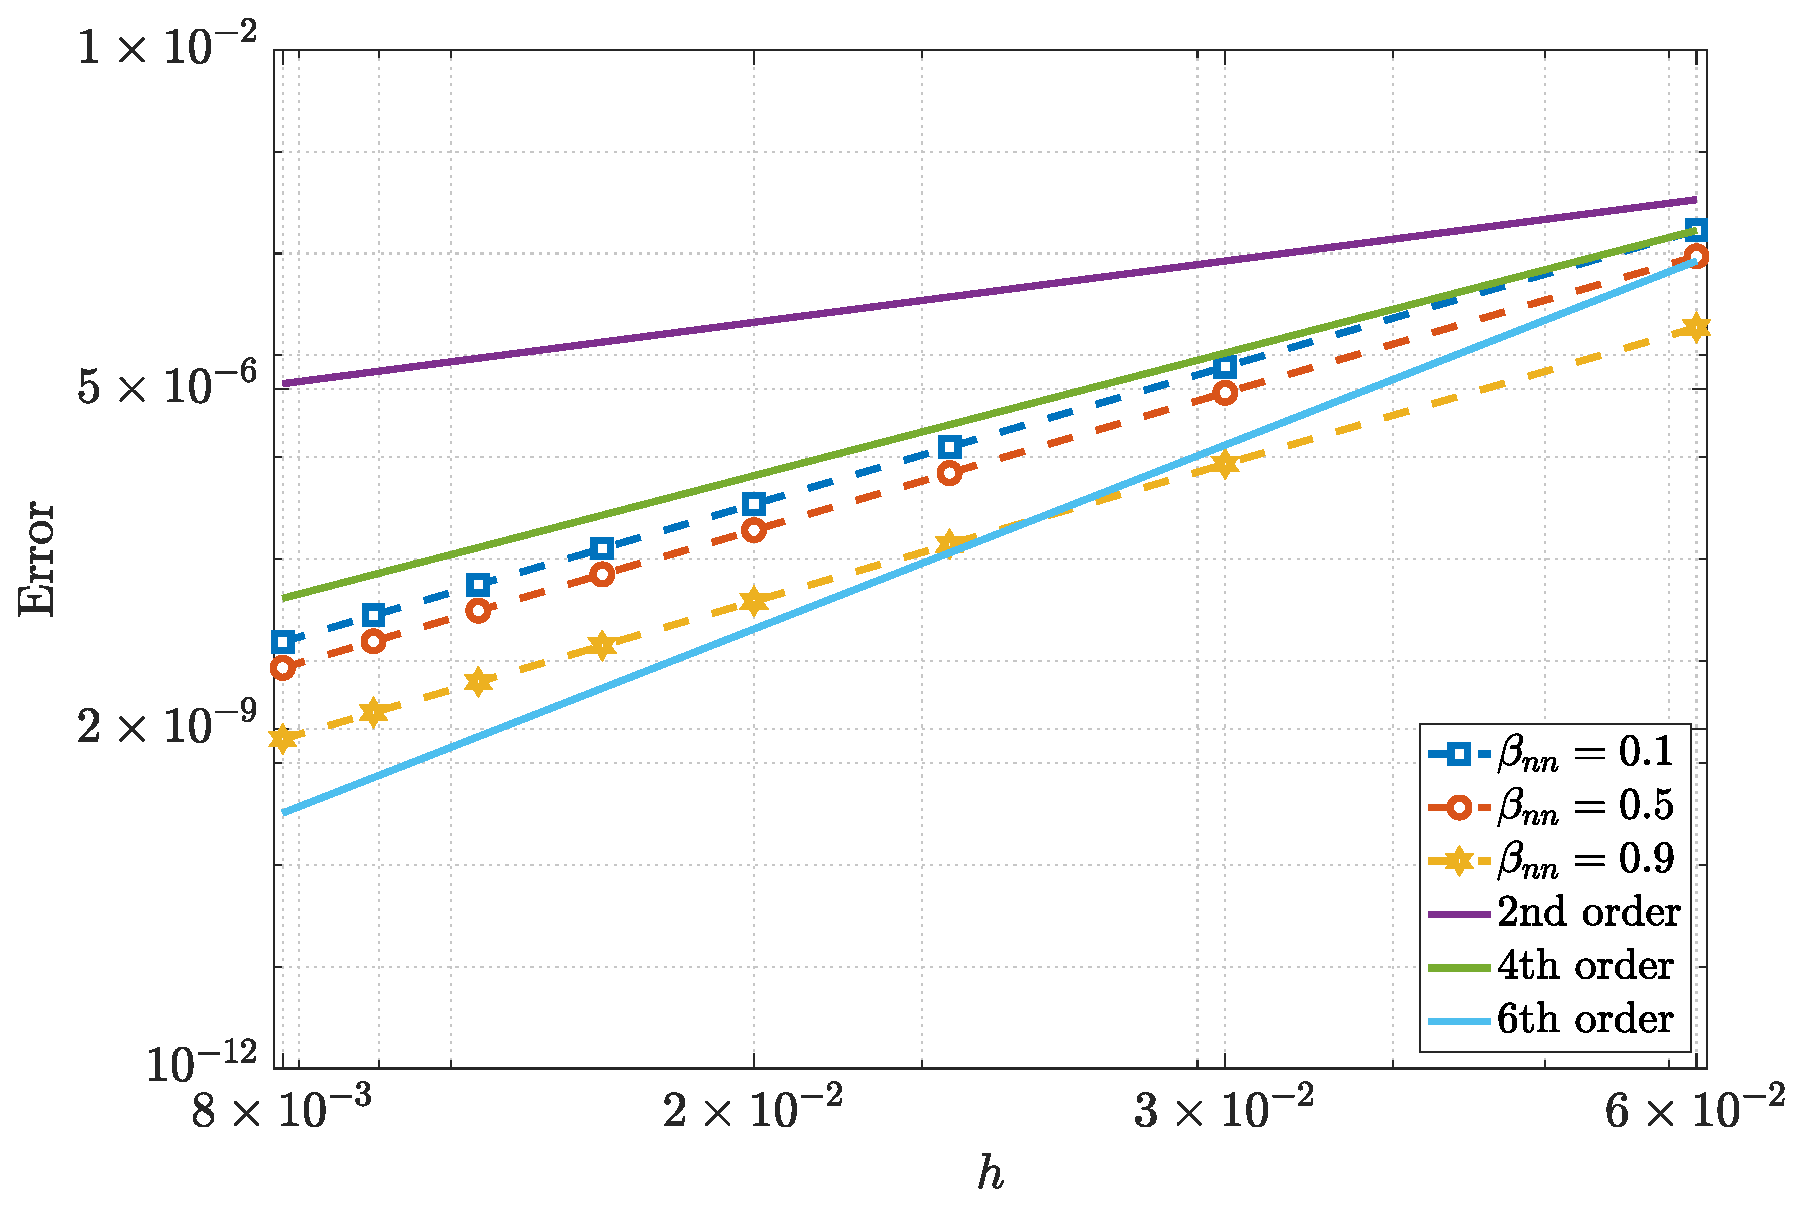
\includegraphics[width=\textwidth]{Figures/NormErr_2nd_Re_100_Wi_1_epsilon_0_xi_0_alphaG_0.1_Dt_1e-06_at_0.05_tipsim_1_MMS_12_Txy.eps}
        \captionof{subfigure}{$\overline{T_{xy}}$}
        \label{giesekus_txy_Case11}
    \end{minipage}
    \hfill
    \begin{minipage}{0.325\textwidth}
        \centering
        \includegraphics[width=\textwidth]{Figures/NormErr_2nd_Re_100_Wi_1_epsilon_0_xi_0_alphaG_0.1_Dt_1e-06_at_0.05_tipsim_1_MMS_12_Tyy.eps}
        \captionof{subfigure}{$\overline{T_{yy}}$}
        \label{giesekus_tyy_Case11}
    \end{minipage}
\end{frame}

%%%%%%%%%%%%%%%%%%%%%%%%%%%%%%%%%%%%%%%%%%%%%%%%%%%%%%%%%%%%%%
\begin{frame}{Caso de verificação usando o modelo LPTT}
    \centering
    \begin{table}[H]
\caption{Erros numéricos e cálculo da ordem de convergência para a vorticidade $(\omega_{z})$, utilizando o parâmetro $Wi=1$, para o escoamento de fluido viscoelástico LPTT.\label{tab_LPTTWzResumida_2}}
\scriptsize{
    \begin{tabular*}{\textwidth}{@{\extracolsep\fill}cccccccccc@{}}
    \hline
    \multirow{2}{*}{$\operatorname{Re}$} & \multirow{2}{*}{Malha} & \multicolumn{2}{c}{$\beta_{nn}=0.1$}  & \multicolumn{2}{c}{$\beta_{nn}=0.5$}  & \multicolumn{2}{c}{$\beta_{nn}=0.9$}  & \multicolumn{2}{c}{$\beta_{nn}=1.0$}\\ %\cline{2-10}
     & & Erro & Ordem & Erro & Ordem & Erro & Ordem & Erro & Ordem \\
    \hline
    \multirow{10}{*}{1.00} & $17\times 17$ & 3.02e-03 & --- & 2.77e-03 & --- & 2.57e-03 & --- & 2.52e-03 & --- \\
    & $33\times 33$ & 2.54e-04 & 3.57 & 1.70e-04 & 4.03 & 1.35e-04 & 4.25 & 1.29e-04 & 4.29 \\
    & $49\times 49$ & 4.87e-05 & 4.07 & 2.59e-05 & 4.64 & 1.99e-05 & 4.72 & 1.90e-05 & 4.73 \\
    & $65\times 65$ & 1.32e-05 & 4.53 & 6.41e-06 & 4.85 & 4.91e-06 & 4.86 & 4.68e-06 & 4.86 \\
    & $81\times 81$ & 4.46e-06 & 4.87 & 2.14e-06 & 4.91 & 1.67e-06 & 4.84 & 1.60e-06 & 4.81 \\
    & $97\times 97$ & 1.76e-06 & 5.09 & 8.69e-07 & 4.95 & 6.98e-07 & 4.77 & 6.76e-07 & 4.72 \\
    & $113\times 133$ & 7.91e-07 & 5.20 & 4.11e-07 & 4.86 & 3.46e-07 & 4.55 & 3.38e-07 & 4.50 \\
    & $129\times 129$ & 4.07e-07 & 4.98 & 2.39e-07 & 4.05 & 2.14e-07 & 3.61 & 2.11e-07 & 3.54 \\
    \hline
    \multirow{10}{*}{100.00} & $17\times 17$ & 3.10e-03 & --- & 3.09e-03 & --- & 3.08e-03 & --- & 3.08e-03 & --- \\
    & $33\times 33$ & 2.93e-04 & 3.40 & 2.91e-04 & 3.41 & 2.88e-04 & 3.42 & 2.88e-04 & 3.42 \\
    & $49\times 49$ & 6.76e-05 & 3.62 & 6.65e-05 & 3.64 & 6.54e-05 & 3.66 & 6.51e-05 & 3.66 \\
    & $65\times 65$ & 2.30e-05 & 3.75 & 2.23e-05 & 3.79 & 2.17e-05 & 3.83 & 2.16e-05 & 3.84 \\
    & $81\times 81$ & 9.72e-06 & 3.86 & 9.28e-06 & 3.93 & 8.88e-06 & 4.01 & 8.79e-06 & 4.02 \\
    & $97\times 97$ & 4.66e-06 & 4.03 & 4.36e-06 & 4.14 & 4.09e-06 & 4.25 & 4.03e-06 & 4.27 \\
    & $113\times 133$ & 2.42e-06 & 4.25 & 2.21e-06 & 4.41 & 2.03e-06 & 4.55 & 1.99e-06 & 4.58 \\
    & $129\times 129$ & 1.38e-06 & 4.22 & 1.22e-06 & 4.46 & 1.09e-06 & 4.67 & 1.06e-06 & 4.71 \\
    \hline
    \end{tabular*}
}
\end{table}
\end{frame}


%%%%%%%%%%%%%%%%%%%%%%%%%%%%%%%%%%%%%%%%%%%%%%%%%%%%%%%%%%%%%%
\begin{frame}{Caso de verificação usando o modelo LPTT}
    \centering
    \begin{table}[H]
\caption{Erros numéricos e cálculo da ordem de convergência para a vorticidade $(\omega_{z})$, utilizando o parâmetro $Wi=1$, para o escoamento de fluido viscoelástico LPTT.\label{tab_LPTTWzResumida_1}}
\scriptsize{
    \begin{tabular*}{\textwidth}{@{\extracolsep\fill}cccccccccc@{}}
    \hline
    \multirow{2}{*}{$\operatorname{Re}$} & \multirow{2}{*}{Malha} & \multicolumn{2}{c}{$\beta_{nn}=0.1$}  & \multicolumn{2}{c}{$\beta_{nn}=0.5$}  & \multicolumn{2}{c}{$\beta_{nn}=0.9$}  & \multicolumn{2}{c}{$\beta_{nn}=1.0$}\\ %\cline{2-10}
     & & Erro & Ordem & Erro & Ordem & Erro & Ordem & Erro & Ordem \\
    \hline
    \multirow{10}{*}{400.00} & $17\times 17$ & 3.10e-03 & --- & 3.09e-03 & --- & 3.08e-03 & --- & 3.08e-03 & --- \\
    & $33\times 33$ & 2.93e-04 & 3.40 & 2.92e-04 & 3.40 & 2.91e-04 & 3.40 & 2.91e-04 & 3.40 \\
    & $49\times 49$ & 6.78e-05 & 3.61 & 6.74e-05 & 3.62 & 6.71e-05 & 3.62 & 6.70e-05 & 3.62 \\
    & $65\times 65$ & 2.31e-05 & 3.74 & 2.29e-05 & 3.75 & 2.28e-05 & 3.76 & 2.27e-05 & 3.76 \\
    & $81\times 81$ & 9.81e-06 & 3.84 & 9.69e-06 & 3.86 & 9.58e-06 & 3.88 & 9.55e-06 & 3.88 \\
    & $97\times 97$ & 4.72e-06 & 4.01 & 4.64e-06 & 4.03 & 4.57e-06 & 4.06 & 4.55e-06 & 4.06 \\
    & $113\times 133$ & 2.47e-06 & 4.21 & 2.41e-06 & 4.25 & 2.36e-06 & 4.28 & 2.35e-06 & 4.29 \\
    & $129\times 129$ & 1.42e-06 & 4.16 & 1.37e-06 & 4.22 & 1.33e-06 & 4.27 & 1.33e-06 & 4.28 \\
    \hline
    \multirow{10}{*}{1000.00} & $17\times 17$ & 3.10e-03 & --- & 3.09e-03 & --- & 3.09e-03 & --- & 3.08e-03 & --- \\
    & $33\times 33$ & 2.93e-04 & 3.40 & 2.93e-04 & 3.40 & 2.92e-04 & 3.40 & 2.92e-04 & 3.40 \\
    & $49\times 49$ & 6.78e-05 & 3.61 & 6.76e-05 & 3.61 & 6.74e-05 & 3.61 & 6.74e-05 & 3.61 \\
    & $65\times 65$ & 2.32e-05 & 3.73 & 2.31e-05 & 3.74 & 2.30e-05 & 3.74 & 2.30e-05 & 3.74 \\
    & $81\times 81$ & 9.84e-06 & 3.84 & 9.78e-06 & 3.85 & 9.73e-06 & 3.85 & 9.72e-06 & 3.85 \\
    & $97\times 97$ & 4.75e-06 & 4.00 & 4.71e-06 & 4.01 & 4.68e-06 & 4.02 & 4.67e-06 & 4.02 \\
    & $113\times 133$ & 2.49e-06 & 4.19 & 2.46e-06 & 4.21 & 2.44e-06 & 4.23 & 2.43e-06 & 4.23 \\
    & $129\times 129$ & 1.43e-06 & 4.13 & 1.41e-06 & 4.16 & 1.39e-06 & 4.18 & 1.39e-06 & 4.18 \\
    \hline
    \end{tabular*}
}
\end{table}
\end{frame}

%%%%%%%%%%%%%%%%%%%%%%%%%%%%%%%%%%%%%%%%%%%%%%%%%%%%%%%%%%%%%%
\begin{frame}{Caso de verificação usando o modelo LPTT}
    \centering
    \captionsetup{justification=centering}
    \captionof{figure}{Erro para o campo de velocidades $(\overline{u},\tilde{v})$ utilizando $Re=100$, $Wi=1$, $\epsilon = 0.5$ e $\xi = 0.1$ para o escoamento de fluido viscoelástico como o modelo LPTT}
    \label{fig:lptt_1}
    \begin{minipage}{0.49\textwidth}
        \centering
        \includegraphics[width=\textwidth]{Figures/NormErr_2nd_Re_100_Wi_1_epsilon_0_xi_0_alphaG_0_Dt_1e-06_at_0.05_tipsim_1_MMS_12_U.eps}
        \captionof{subfigure}{$\overline{u}$}
        \label{lptt_u_Case11}
    \end{minipage}
    \hfill
    \begin{minipage}{0.49\textwidth}
        \centering
        \includegraphics[width=\textwidth]{Figures/NormErr_2nd_Re_100_Wi_1_epsilon_0_xi_0_alphaG_0_Dt_1e-06_at_0.05_tipsim_1_MMS_12_V.eps}
        \captionof{subfigure}{$\tilde{v}$}
        \label{lptt_v_Case11}
    \end{minipage}
\end{frame}

%%%%%%%%%%%%%%%%%%%%%%%%%%%%%%%%%%%%%%%%%%%%%%%%%%%%%%%%%%%%%%
\begin{frame}{Caso de verificação usando o modelo LPTT}
    \centering
    \captionsetup{justification=centering}
    \captionof{figure}{Erro para a vorticidade $(\tilde{\omega_{z}})$ e função de corrente $(\tilde{\psi})$, utilizando $Re=100$, $Wi=1$, $\epsilon = 0.5$ e $\xi = 0.1$ para o escoamento de fluido viscoelástico como o modelo LPTT}
    \label{fig:lptt_2}
    \begin{minipage}{0.49\textwidth}
        \centering
        \includegraphics[width=\textwidth]{Figures/NormErr_2nd_Re_100_Wi_1_epsilon_0_xi_0_alphaG_0_Dt_1e-06_at_0.05_tipsim_1_MMS_12_Wz.eps}
        \captionof{subfigure}{$\tilde{\omega_{z}}$}
        \label{lptt_wz_Case11}
    \end{minipage}
    \hfill
    \begin{minipage}{0.49\textwidth}
        \centering
        \includegraphics[width=\textwidth]{Figures/NormErr_2nd_Re_100_Wi_1_epsilon_0_xi_0_alphaG_0_Dt_1e-06_at_0.05_tipsim_1_MMS_12_Psi.eps}
        \captionof{subfigure}{$\tilde{\psi}$}
        \label{lptt_psi_Case11}
    \end{minipage}
\end{frame}

%%%%%%%%%%%%%%%%%%%%%%%%%%%%%%%%%%%%%%%%%%%%%%%%%%%%%%%%%%%%%%
\begin{frame}{Caso de verificação usando o modelo LPTT}
    \centering
    \captionsetup{justification=centering}
    \captionof{figure}{Erro para as componentes dos tensores de tensões, utilizando $Re=100$, $Wi=1$, $\epsilon = 0.5$ e $\xi = 0.1$ para o escoamento de fluido viscoelástico como o modelo LPTT}
    \label{fig:lptt_3}
    \begin{minipage}{0.325\textwidth}
        \centering
        \includegraphics[width=\textwidth]{Figures/NormErr_2nd_Re_100_Wi_1_epsilon_0_xi_0_alphaG_0_Dt_1e-06_at_0.05_tipsim_1_MMS_12_Psi.eps}
        \captionof{subfigure}{$\overline{T_{xx}}$}
        \label{lptt_txx_Case11}
    \end{minipage}
    \hfill
    \begin{minipage}{0.325\textwidth}
        \centering
        \includegraphics[width=\textwidth]{Figures/NormErr_2nd_Re_100_Wi_1_epsilon_0_xi_0_alphaG_0_Dt_1e-06_at_0.05_tipsim_1_MMS_12_Txy.eps}
        \captionof{subfigure}{$\overline{T_{xy}}$}
        \label{lptt_txy_Case11}
    \end{minipage}
    \hfill
    \begin{minipage}{0.325\textwidth}
        \centering
        \includegraphics[width=\textwidth]{Figures/NormErr_2nd_Re_100_Wi_1_epsilon_0_xi_0_alphaG_0_Dt_1e-06_at_0.05_tipsim_1_MMS_12_Tyy.eps}
        \captionof{subfigure}{$\overline{T_{yy}}$}
        \label{lptt_tyy_Case11}
    \end{minipage}
\end{frame}

%%%%%%%%%%%%%%%%%%%%%%%%%%%%%%%%%%%%%%%%%%%%%%%%%%%%%%%%%%%%%%
\subsection{Considerações finais}
%%%%%%%%%%%%%%%%%%%%%%%%%%%%%%%%%%%%%%%%%%%%%%%%%%%%%%%%%%%%%%
%%%%%%%%%%%%%%%%%%%%%%%%%%%%%%%%%%%%%%%%%%%%%%%%%%%%%%%%%%%%%%

\begin{frame}{Conclusões}
\begin{itemize}
    \item O estudo reforça a eficácia dos métodos numéricos na simulação de fluidos viscoelásticos;
    \item Simulações para diversos números de Reynolds ($Re$) e Weissenberg ($Wi$), além de razões de viscosidade do solvente ($\beta_{nn}$), validaram a robustez dos modelos;
    \item O modelo UCM apresentou precisão elevada para fenômenos de elasticidade em malhas refinadas;
    \item O modelo LPTT demonstrou estabilidade e precisão para diferentes valores do parâmetro $\epsilon$;
    \item Fluidos Newtonianos ($\beta_{nn}=1$) atingiram erros próximos à precisão de máquina, validando os esquemas numéricos;
    \item O modelo Oldroyd-B mostrou-se robusto e preciso, enquanto o modelo Giesekus manteve estabilidade para valores de $\alpha_G$ variando entre 0.1 e 0.5;
    \item O Método das Soluções Manufaturadas se mostrou crucial para a verificação de códigos numéricos;
    \item Os resultados sustentam a aplicação dos modelos UCM, LPTT, Oldroyd-B e Giesekus em cenários complexos de escoamento;
\end{itemize}
\end{frame}

%%%%%%%%%%%%%%%%%%%%%%%%%%%%%%%%%%%%%%%%%%%%%%%%%%%%%%%%%%%%%%
\begin{frame}{Considerações finais e trabalhos futuros}
\begin{itemize}
    \item \textbf{SILVA, A. T. G. et al.} Validation of HiG-Flow Software for Simulating Two-Phase Flows with a 3D Geometric Volume of Fluid Algorithm. \textit{Mathematics}, v. 11, n. 18, p. 3900, 2023. 
\end{itemize}
\end{frame}

%%%%%%%%%%%%%%%%%%%%%%%%%%%%%%%%%%%%%%%%%%%%%%%%%%
\section{Referências e agradecimentos}
%%%%%%%%%%%%%%%%%%%%%%%%%%%%%%%%%%%%%%%%%%%%%%%%%%

%%%%%%%%%%%%%%%%%%%%%%%%%%%%%%%%%%%%%%%%%%%%%%%%%%
\begin{frame}[allowframebreaks]
	\frametitle{Referências}
        \bibliographystyle{plainnat}
	\bibliography{referencesOrganistaJ}
\end{frame}

%%%%%%%%%%%%%%%%%%%%%%%%%%%%%%%%%%%%%%%%%%%%%%%%%%
\begin{frame}{Agradecimentos}
\color{fg} 
\noindent
\begin{center}
	\begin{Large}
		Obrigada pela atenção!
	\end{Large}
\end{center}
\vspace{1cm}
\begin{center}
	\begin{Large}
		Perguntas!?
	\end{Large}
\end{center}
\vspace{-2.5cm}
\begin{columns} 
\column{0.51\textwidth}
\vskip 1cm
   
\includegraphics[scale=0.33]{AAUgraphics/agrad.eps}
 \column{0.51 \textwidth}
 \begin{flushright}
\begin{minipage}{0.8\textwidth}
\vskip 3cm
\end{minipage}
\end{flushright}
\end{columns} 
\end{frame}

\end{document}
